%%%%%%%%%%%%PREAMBLE%%%%%%%%%%%%
\documentclass{report}
\usepackage[utf8]{inputenc}
\usepackage[english]{babel}
\usepackage{enumerate}
\usepackage[margin=1in]{geometry}
\usepackage{hyperref}
% code
\usepackage{color}
\usepackage{xcolor}
\usepackage{listings}
%\usepackage{minted}
%\usepackage{attachfile}
%\usepackage{accsupp}
%\usepackage{verbatim}
%\usepackage[misc]{ifsym}

% math
\usepackage{amsfonts}
%\usepackage{amssymb}
%\usepackage{amsmath}
%\usepackage{amsthm}

% graphics
\usepackage{float}
\usepackage{graphicx}
%\usepackage{pgfplot}
%\usepackage{fancyhdr}
\usepackage{tikz}
% https://users.ece.utexas.edu/~garg/dist/listings.pdf
% Taken from Lena Herrmann at 
% http://lenaherrmann.net/2010/05/20/javascript-syntax-highlighting-in-the-latex-listings-package
\definecolor{lightgray}{rgb}{.9,.9,.9}
\definecolor{darkgray}{rgb}{.4,.4,.4}
\definecolor{purple}{rgb}{0.65, 0.12, 0.82}
\definecolor{background}{HTML}{EEEEEE}
\colorlet{punct}{red!60!black}
\definecolor{background}{HTML}{EEEEEE}
\definecolor{delim}{RGB}{20,105,176}
\colorlet{numb}{magenta!60!black}

\lstdefinelanguage{Typescript}{
  keywords={typeof, new, true, false, catch, function, return, null, catch, switch, var, if, in, while, do, else, case, break},
  keywordstyle=\color{blue}\bfseries,
  ndkeywords={class, export, boolean, throw, implements, import, this},
  ndkeywordstyle=\color{darkgray}\bfseries,
  identifierstyle=\color{black},
  sensitive=false,
  comment=[l]{//},
  morecomment=[s]{/*}{*/},
  commentstyle=\color{purple}\ttfamily,
  stringstyle=\color{red}\ttfamily,
  morestring=[b]',
  morestring=[b]"
}

\lstdefinelanguage{json}{
	basicstyle=\normalfont\ttfamily,
	numbers=left,
	numberstyle=\scriptsize,
	stepnumber=1,
	numbersep=8pt,
	showstringspaces=false,
	breaklines=true,
	frame=lines,
	backgroundcolor=\color{background},
	literate=
	*{0}{{{\color{numb}0}}}{1}
	{1}{{{\color{numb}1}}}{1}
	{2}{{{\color{numb}2}}}{1}
	{3}{{{\color{numb}3}}}{1}
	{4}{{{\color{numb}4}}}{1}
	{5}{{{\color{numb}5}}}{1}
	{6}{{{\color{numb}6}}}{1}
	{7}{{{\color{numb}7}}}{1}
	{8}{{{\color{numb}8}}}{1}
	{9}{{{\color{numb}9}}}{1}
	{:}{{{\color{punct}{:}}}}{1}
	{,}{{{\color{punct}{,}}}}{1}
	{\{}{{{\color{delim}{\{}}}}{1}
	{\}}{{{\color{delim}{\}}}}}{1}
	{[}{{{\color{delim}{[}}}}{1}
	{]}{{{\color{delim}{]}}}}{1},
}

\lstdefinelanguage{HTML5}{
	language=html,
	sensitive=true, 
	alsoletter={<>=-},
	otherkeywords={
		% HTML tags
		<, </, >,
		</a, <a, </a>,
		</abbr, <abbr, </abbr>,
		</address, <address, </address>,
		</area, <area, </area>,
		</area, <area, </area>,
		</article, <article, </article>,
		</aside, <aside, </aside>,
		</audio, <audio, </audio>,
		</audio, <audio, </audio>,
		</b, <b, </b>,
		</base, <base, </base>,
		</bdi, <bdi, </bdi>,
		</bdo, <bdo, </bdo>,
		</blockquote, <blockquote, </blockquote>,
		</body, <body, </body>,
		</br, <br, </br>,
		</button, <button, </button>,
		</canvas, <canvas, </canvas>,
		</caption, <caption, </caption>,
		</cite, <cite, </cite>,
		</code, <code, </code>,
		</col, <col, </col>,
		</colgroup, <colgroup, </colgroup>,
		</data, <data, </data>,
		</datalist, <datalist, </datalist>,
		</dd, <dd, </dd>,
		</del, <del, </del>,
		</details, <details, </details>,
		</dfn, <dfn, </dfn>,
		</div, <div, </div>,
		</dl, <dl, </dl>,
		</dt, <dt, </dt>,
		</em, <em, </em>,
		</embed, <embed, </embed>,
		</fieldset, <fieldset, </fieldset>,
		</figcaption, <figcaption, </figcaption>,
		</figure, <figure, </figure>,
		</footer, <footer, </footer>,
		</form, <form, </form>,
		</h1, <h1, </h1>,
		</h2, <h2, </h2>,
		</h3, <h3, </h3>,
		</h4, <h4, </h4>,
		</h5, <h5, </h5>,
		</h6, <h6, </h6>,
		</head, <head, </head>,
		</header, <header, </header>,
		</hr, <hr, </hr>,
		</html, <html, </html>,
		</i, <i, </i>,
		</iframe, <iframe, </iframe>,
		</img, <img, </img>,
		</input, <input, </input>,
		</ins, <ins, </ins>,
		</kbd, <kbd, </kbd>,
		</keygen, <keygen, </keygen>,
		</label, <label, </label>,
		</legend, <legend, </legend>,
		</li, <li, </li>,
		</link, <link, </link>,
		</main, <main, </main>,
		</map, <map, </map>,
		</mark, <mark, </mark>,
		</math, <math, </math>,
		</menu, <menu, </menu>,
		</menuitem, <menuitem, </menuitem>,
		</meta, <meta, </meta>,
		</meter, <meter, </meter>,
		</nav, <nav, </nav>,
		</noscript, <noscript, </noscript>,
		</object, <object, </object>,
		</ol, <ol, </ol>,
		</optgroup, <optgroup, </optgroup>,
		</option, <option, </option>,
		</output, <output, </output>,
		</p, <p, </p>,
		</param, <param, </param>,
		</pre, <pre, </pre>,
		</progress, <progress, </progress>,
		</q, <q, </q>,
		</rp, <rp, </rp>,
		</rt, <rt, </rt>,
		</ruby, <ruby, </ruby>,
		</s, <s, </s>,
		</samp, <samp, </samp>,
		</script, <script, </script>,
		</section, <section, </section>,
		</select, <select, </select>,
		</small, <small, </small>,
		</source, <source, </source>,
		</span, <span, </span>,
		</strong, <strong, </strong>,
		</style, <style, </style>,
		</summary, <summary, </summary>,
		</sup, <sup, </sup>,
		</svg, <svg, </svg>,
		</table, <table, </table>,
		</tbody, <tbody, </tbody>,
		</td, <td, </td>,
		</template, <template, </template>,
		</textarea, <textarea, </textarea>,
		</tfoot, <tfoot, </tfoot>,
		</th, <th, </th>,
		</thead, <thead, </thead>,
		</time, <time, </time>,
		</title, <title, </title>,
		</tr, <tr, </tr>,
		</track, <track, </track>,
		</u, <u, </u>,
		</ul, <ul, </ul>,
		</var, <var, </var>,
		</video, <video, </video>,
		</wbr, <wbr, </wbr>,
		/>, <!
	},  
	ndkeywords={
		% General
		=,
		% HTML attributes
		accept=, accept-charset=, accesskey=, action=, align=, alt=, async=, autocomplete=, autofocus=, autoplay=, autosave=, bgcolor=, border=, buffered=, challenge=, charset=, checked=, cite=, class=, code=, codebase=, color=, cols=, colspan=, content=, contenteditable=, contextmenu=, controls=, coords=, data=, datetime=, default=, defer=, dir=, dirname=, disabled=, download=, draggable=, dropzone=, enctype=, for=, form=, formaction=, headers=, height=, hidden=, high=, href=, hreflang=, http-equiv=, icon=, id=, ismap=, itemprop=, keytype=, kind=, label=, lang=, language=, list=, loop=, low=, manifest=, max=, maxlength=, media=, method=, min=, multiple=, name=, novalidate=, open=, optimum=, pattern=, ping=, placeholder=, poster=, preload=, pubdate=, radiogroup=, readonly=, rel=, required=, reversed=, rows=, rowspan=, sandbox=, scope=, scoped=, seamless=, selected=, shape=, size=, sizes=, span=, spellcheck=, src=, srcdoc=, srclang=, start=, step=, style=, summary=, tabindex=, target=, title=, type=, usemap=, value=, width=, wrap=,
		% CSS properties
		accelerator:,azimuth:,background:,background-attachment:,
		background-color:,background-image:,background-position:,
		background-position-x:,background-position-y:,background-repeat:,
		behavior:,border:,border-bottom:,border-bottom-color:,
		border-bottom-style:,border-bottom-width:,border-collapse:,
		border-color:,border-left:,border-left-color:,border-left-style:,
		border-left-width:,border-right:,border-right-color:,
		border-right-style:,border-right-width:,border-spacing:,
		border-style:,border-top:,border-top-color:,border-top-style:,
		border-top-width:,border-width:,bottom:,caption-side:,clear:,
		clip:,color:,content:,counter-increment:,counter-reset:,cue:,
		cue-after:,cue-before:,cursor:,direction:,display:,elevation:,
		empty-cells:,filter:,float:,font:,font-family:,font-size:,
		font-size-adjust:,font-stretch:,font-style:,font-variant:,
		font-weight:,height:,ime-mode:,include-source:,
		layer-background-color:,layer-background-image:,layout-flow:,
		layout-grid:,layout-grid-char:,layout-grid-char-spacing:,
		layout-grid-line:,layout-grid-mode:,layout-grid-type:,left:,
		letter-spacing:,line-break:,line-height:,list-style:,
		list-style-image:,list-style-position:,list-style-type:,margin:,
		margin-bottom:,margin-left:,margin-right:,margin-top:,
		marker-offset:,marks:,max-height:,max-width:,min-height:,
		min-width:,transition-duration:,transition-property:,
		transition-timing-function:,transform:,
		-moz-transform:,-moz-binding:,-moz-border-radius:,
		-moz-border-radius-topleft:,-moz-border-radius-topright:,
		-moz-border-radius-bottomright:,-moz-border-radius-bottomleft:,
		-moz-border-top-colors:,-moz-border-right-colors:,
		-moz-border-bottom-colors:,-moz-border-left-colors:,-moz-opacity:,
		-moz-outline:,-moz-outline-color:,-moz-outline-style:,
		-moz-outline-width:,-moz-user-focus:,-moz-user-input:,
		-moz-user-modify:,-moz-user-select:,orphans:,outline:,
		outline-color:,outline-style:,outline-width:,overflow:,
		overflow-X:,overflow-Y:,padding:,padding-bottom:,padding-left:,
		padding-right:,padding-top:,page:,page-break-after:,
		page-break-before:,page-break-inside:,pause:,pause-after:,
		pause-before:,pitch:,pitch-range:,play-during:,position:,quotes:,
		-replace:,richness:,right:,ruby-align:,ruby-overhang:,
		ruby-position:,-set-link-source:,size:,speak:,speak-header:,
		speak-numeral:,speak-punctuation:,speech-rate:,stress:,
		scrollbar-arrow-color:,scrollbar-base-color:,
		scrollbar-dark-shadow-color:,scrollbar-face-color:,
		scrollbar-highlight-color:,scrollbar-shadow-color:,
		scrollbar-3d-light-color:,scrollbar-track-color:,table-layout:,
		text-align:,text-align-last:,text-decoration:,text-indent:,
		text-justify:,text-overflow:,text-shadow:,text-transform:,
		text-autospace:,text-kashida-space:,text-underline-position:,top:,
		unicode-bidi:,-use-link-source:,vertical-align:,visibility:,
		voice-family:,volume:,white-space:,widows:,width:,word-break:,
		word-spacing:,word-wrap:,writing-mode:,z-index:,zoom:
	},  
	morecomment=[s]{<!--}{-->},
	tag=[s]
}

\lstdefinelanguage{CSS}{
	keywords={accelerator,azimuth,background,background-attachment,
		background-color,background-image,background-position,
		background-position-x,background-position-y,background-repeat,
		behavior,border,border-bottom,border-bottom-color,
		border-bottom-style,border-bottom-width,border-collapse,
		border-color,border-left,border-left-color,border-left-style,
		border-left-width,border-right,border-right-color,
		border-right-style,border-right-width,border-spacing,
		border-style,border-top,border-top-color,border-top-style,
		border-top-width,border-width,bottom,caption-side,clear,
		clip,color,content,counter-increment,counter-reset,cue,
		cue-after,cue-before,cursor,direction,display,elevation,
		empty-cells,filter,float,font,font-family,font-size,
		font-size-adjust,font-stretch,font-style,font-variant,
		font-weight,height,ime-mode,include-source,
		layer-background-color,layer-background-image,layout-flow,
		layout-grid,layout-grid-char,layout-grid-char-spacing,
		layout-grid-line,layout-grid-mode,layout-grid-type,left,
		letter-spacing,line-break,line-height,list-style,
		list-style-image,list-style-position,list-style-type,margin,
		margin-bottom,margin-left,margin-right,margin-top,
		marker-offset,marks,max-height,max-width,min-height,
		min-width,-moz-binding,-moz-border-radius,
		-moz-border-radius-topleft,-moz-border-radius-topright,
		-moz-border-radius-bottomright,-moz-border-radius-bottomleft,
		-moz-border-top-colors,-moz-border-right-colors,
		-moz-border-bottom-colors,-moz-border-left-colors,-moz-opacity,
		-moz-outline,-moz-outline-color,-moz-outline-style,
		-moz-outline-width,-moz-user-focus,-moz-user-input,
		-moz-user-modify,-moz-user-select,orphans,outline,
		outline-color,outline-style,outline-width,overflow,
		overflow-X,overflow-Y,padding,padding-bottom,padding-left,
		padding-right,padding-top,page,page-break-after,
		page-break-before,page-break-inside,pause,pause-after,
		pause-before,pitch,pitch-range,play-during,position,quotes,
		-replace,richness,right,ruby-align,ruby-overhang,
		ruby-position,-set-link-source,size,speak,speak-header,
		speak-numeral,speak-punctuation,speech-rate,stress,
		scrollbar-arrow-color,scrollbar-base-color,
		scrollbar-dark-shadow-color,scrollbar-face-color,
		scrollbar-highlight-color,scrollbar-shadow-color,
		scrollbar-3d-light-color,scrollbar-track-color,table-layout,
		text-align,text-align-last,text-decoration,text-indent,
		text-justify,text-overflow,text-shadow,text-transform,
		text-autospace,text-kashida-space,text-underline-position,top,
		unicode-bidi,-use-link-source,vertical-align,visibility,
		voice-family,volume,white-space,widows,width,word-break,
	word-spacing,word-wrap,writing-mode,z-index,zoom},  
	sensitive=true,
	morecomment=[l]{//},
	morecomment=[s]{/*}{*/},
	morestring=[b]',
	morestring=[b]",
	alsoletter={:},
	alsodigit={-}
}

%\definecolor{codegreen}{rgb}{0,0.6,0}
%\definecolor{codegray}{rgb}{0.5,0.5,0.5}
%\definecolor{codepurple}{rgb}{0.58,0,0.82}
%\definecolor{backcolour}{rgb}{0.95,0.95,0.92}
%
%\lstdefinestyle{mystyle}{
%    backgroundcolor=\color{backcolour},   
%    commentstyle=\color{codegreen},
%    keywordstyle=\color{magenta},
%    numberstyle=\tiny\color{codegray},
%    stringstyle=\color{codepurple},
%    basicstyle=\ttfamily\footnotesize,
%    breakatwhitespace=false,         
%    breaklines=true,                 
%    captionpos=b,                    
%    keepspaces=true,                 
%    numbers=left,                    
%    numbersep=5pt,                  
%    showspaces=false,                
%    showstringspaces=false,
%    showtabs=false,                  
%    tabsize=2
%}

%\lstset{style=mystyle}
\lstset{ 
	%frame=TRBL,
	frame=shadowbox,
	frameround=ffft,
	rulesepcolor=\color{purple},
	tabsize=2,
	framexleftmargin=6mm,
	numbers=left,
	breaklines=true,
	extendedchars=true,
	basicstyle=\footnotesize\ttfamily,
	showstringspaces=false,
	backgroundcolor=\color{lightgray},
	showspaces=false,
	columns=fullflexible,
	captionpos=b,
	postbreak=\mbox{\textcolor{red}{$\hookrightarrow$}\space}
}

\title{\textbf{Angular}: Beyond Basics}
\author{Mimanshu Maheshwari}
\date{\today}

%\pagestyle{fancy}
%\fancyhead[l]{Mimanshu Maheshwari}
%\fancyhead[r]{\today}
%\fancyhead[c]{\thepage}
%\fancyfoot[l]{Mimanshu Maheshwari}
%\fancyfoot[r]{\today}
%\fancyfoot[c]{\thepage}
%\renewcommand{\headrulewidth}{0.2pt}
%\setlength{\headheight}{15pt}


%%%%%%%%%%%%END%%%%%%%%%%%%



\begin{document}

\maketitle
\tableofcontents
%\listoftables
\listoffigures
%\listoffigures

\chapter{Content Projection}
\section{Introduction}
In this context, having data-driven DOM structures prove to be extremely helpful as one directive or component can be created such that it will allow to insert data dynamically.
This brings in reusability, minimizing the time, effort and duplication of code thereby minimizing the need of re-designing any part of the application that is already created. 

Content Projection in Angular is a powerful and flexible way to create reusable components with dynamic content.
It facilitates passing content from a parent component to a child component.
This makes it possible to insert content dynamically into a component’s template from the outside.
Content Projection is also known as \textbf{Transclusion}. 

Content projection helps in padding the data types that cannot be passed with the @Input decorator:  
\begin{itemize}
	\item Inner HTML
	\item HTML Elements
	\item Styed HTML
	\item Other Components
\end{itemize}
Content Projection has three flavours: 
\begin{itemize}
	\item Single slot Content Projection
	\item Multi slot Content Projection
	\item Conditional Content Projection
\end{itemize}

\section{Single Slot Content Projection}
\begin{itemize}
	\item{In the Parent Component}
		\begin{itemize}
			\item{Define a child component tag in the parent's tmeplate}
			\item{Add content between the opening and closing tag of the child component. This content will be projected into the child component template}
		\end{itemize}
		\begin{lstlisting}[caption=app-parent.component.html,language=HTML]
			<app-child>
			Projected content <!- content to be projected --> 
			</app-child>
	\end{lstlisting}

\item{In the child component}
	\begin{itemize}
		\item{Use \lstinline{<ng-content>} directive to specify where the projcted content should b placed.}
	\end{itemize}
		\begin{lstlisting}[caption=app-child.component.html,language=HTML]
			<div> 
			<h2> Child Component content</h2>
			<h3> Single Slot content projection</h3>
			<ng-content></ng-content>
			</div>
\end{lstlisting}
\end{itemize}
\section{Multi Slot Content Projection}

		\begin{lstlisting}[caption=app-parent.component.html,language=HTML]
			<app-child>
				<div slot="header">Header content</div>
				<div slot="body">Body content</div>
			</app-child>
\end{lstlisting}

		\begin{lstlisting}[caption=app-child.component.html ,language=HTML]
			<div>
				<h3>Multi slot content projection</h3>
				<ng-content></ng-content> <!- Display default content --> 
				<div class="header">
					<ng-content select="[slot=header]"></ng-content> <!- Display specific content -->
				</div> 
				<div class="body">
					<ng-content select="[slot=body]"></ng-content> <!- Display specific content -->
				</div>
			</div>
\end{lstlisting}
\section{Conditional Content Projection}
If the component needs to conditionally render content or has to render content multiple times, then the component shoud accept a \lstinline{<ng-template>} element which can contain the conditionally rendered content.

In these scenarios, usage of \lstinline{<ng-content>} is not advisable. This is because, when the cosumer of the component delivers the content, the content gets initialized always, even if component doesn’t have \lstinline{<ng-content>} or the \lstinline{<ng-content>} is present within an \lstinline{ngIf} statement.

With \lstinline{<ng-template>}, content is not renderd by default by Angular. It needs to be explicitly rendered. So you can render content based on any condition or how many ever times we want. Hence here, \lstinline{<ng-template>} is more preferred over \lstinline{<ng-content>}

\begin{lstlisting}[caption=app.component.ts, language=Typescript]
	@Component({
		selector: 'app-component',
		template: `
			<div *ngIf="isLoggedIn; else loggedOut"> Welcome back </div>
			<ng-template #loggedOut>Please Login!!</ng-template>
			`,
	})
	export class AppComponent{
		isLoggedIn = true;
	}
\end{lstlisting}

\chapter{Dynamic Components}
\section{Introduction}
Consider a scenario where there is a need to build a dynamic ad banne.
Various advertisements need to be displayed in the ad banner.
Fresh ad components get added regularly.
Sticking to a static component structure for AdComponent is hence close to impossible.
Instead, there needs to be some way which can  load a new offer component without a permanent mention to the component in the template of the AdComponent.
This is why Angular introduced the concept of dynamic components.
Dynamic components in Angular allows to generate and render components dynamically at runtime.
This comes in extremely handy in the context of dynamic user interfaces or when there is a need for creation of components based on user interactions. \\
\textbf{The anchor directive} \\
Before considering to add components, an anchor point has to be defined which can act as a guide to Angular for informing where to insert components.

\section{Demo}
The ad banner uses a helper directive named \lstinline{AdDirective} for marking insertion points in the template.

\begin{lstlisting}[caption=ad.directive.ts, language=Typescript]
	import {Directive, ViewContainerRef} from '@angular/core';
	@Directive({
		selector: '[adHost]', 
	})
	export class AdDirective {
		constructor(public viewContainerRef: ViewContainerRef){ }
	}
\end{lstlisting}

The directive will inject ViewContainerRef. This makes it possible for the directive to gain access to the view container of the element that will take care of hosting the dynamically added component.

\begin{lstlisting}[caption=ad.ts, language=Typescript]
	export interface AdComponent {
		data:any;
	}
\end{lstlisting}

A common \lstinline{AdComponent} interface will be implemented by all components. This will help to standardize the API as it needs to pass data to the components. 

\begin{lstlisting}[caption=ad-item.ts, language=Typescript]
	import {Type} from '@angular/core';
	export class AdItem{
		constructor(public component: Type<any>, public data: any){ }
	}
\end{lstlisting}

\lstinline{AdItem} assists in stating the type of component which has to be loaded and the data that has to be bound to the component.

\begin{lstlisting}[caption=ad.service.ts, language=Typescript]

	import { Injectable } from '@angular/core';
	import { AdItem } from './ad-item';
	import { ProfileComponent } from './profile.component';
	import { JobAdComponent } from './job-ad.component';
	@Injectable()
	export class AdService {
		getAds() {
			return [
			new AdItem(
			ProfileComponent,
			{ name: 'Dr. Jack', bio: 'Awesome Cardiac' }
			),
			new AdItem(
			ProfileComponent,
			{ name: 'Dr. Mary', bio: 'Wonderful OB/GYN' }
			),
			new AdItem(
			JobAdComponent,
			{ headline: 'We are hiring for many positions', body: 'Bring in your resume today!' }
			),
			new AdItem(
			JobAdComponent,
			{ headline: 'We have openings in many departments', body: 'Apply today to make the best use of opportunities!' }
			)
			];
		}
	}

\end{lstlisting}

\lstinline{AdService} will returns the actual ads which are required for making the ad campaign. The service’s \lstinline{getAds()} method return an array of \lstinline{AdItem} objects.

\begin{lstlisting}[caption=ad-banner.component.ts, language=Typescript]
	import { Component, Input, OnDestroy, OnInit, ViewChild } from '@angular/core';
	import { AdDirective } from './ad.directive';
	import { AdItem } from './ad-item';
	import { AdComponent } from './ad';
	@Component({
		selector: 'app-ad-banner',
		template: `
		<div class="ad-banner-example">
		<h3>Advertisements Section</h3>
		<hr/>
		<ng-template adHost></ng-template>
		</div>
		`
	})
	export class AdBannerComponent implements OnInit, OnDestroy {
		@Input() ads: AdItem[] = [];
		currentAdIndex = -1;
		@ViewChild(AdDirective, {static: true}) adHost!: AdDirective;
		private clearTimer: VoidFunction | undefined;
		ngOnInit(): void {
			this.loadComponent();
			this.getAds();
		}
		ngOnDestroy() {
			this.clearTimer?.();
		}
		loadComponent() {
			this.currentAdIndex = (this.currentAdIndex + 1) % this.ads.length;
			const adItem = this.ads[this.currentAdIndex];
			const viewContainerRef = this.adHost.viewContainerRef;
			viewContainerRef.clear();
			const componentRef = viewContainerRef.createComponent<AdComponent>(adItem.component);
			componentRef.instance.data = adItem.data;
		}
		getAds() {
			const interval = setInterval(() => {
				this.loadComponent();
			}, 3000);
			this.clearTimer = () => clearInterval(interval);
		}
	}
\end{lstlisting}
Due to the use of \lstinline{<ng-template>} in above code, Angular will know where it has to dynamically load components. The \lstinline{<ng-template>} element is a preferred choice while creating dynamic components as it doesn't lead to rendering of any additional output.

\begin{lstlisting}[caption=job-ad.component.ts, language=Typescript]
	import { Component, Input } from '@angular/core';
	import { AdComponent } from './ad';
	@Component({
		template: `
		<div>
		<h3>Job Opportunities:</h3>
		<h4>{{data.headline}}</h4>
		{{data.body}}
		</div>
		`
	})
	export class JobAdComponent implements AdComponent {
		@Input() data: any;
	}
\end{lstlisting}

\begin{lstlisting}[caption=profile.component.ts, language=Typescript]
	import { Component, Input } from '@angular/core';
	import { AdComponent } from './ad';
	@Component({
		template: `
		<div>
		<h3>Featured Profile:</h3>
		<h4>{{data.name}}</h4>
		<p>{{data.bio}}</p>      
		</div>
		`
	})
	export class ProfileComponent implements AdComponent {
		@Input() data: any;
	}
\end{lstlisting}

\begin{lstlisting}[caption=app.module.ts, language=Typescript]
	import { BrowserModule } from '@angular/platform-browser';
	import { NgModule } from '@angular/core';
	import { AppComponent } from './app.component';
	import { AdBannerComponent } from './ad-banner.component';
	import { AdDirective } from './ad.directive';
	import { AdService } from './ad.service';
	import { JobAdComponent } from './job-ad.component';
	import { ProfileComponent } from './profile.component';
	@NgModule({
		imports: [ BrowserModule ],
		providers: [ AdService ],
		declarations: [
		AppComponent,
		AdBannerComponent,
		JobAdComponent,
		ProfileComponent,
		AdDirective
		],
		bootstrap: [ AppComponent ]
	})
	export class AppModule { }
\end{lstlisting}


\begin{lstlisting}[caption=app.component.ts, language=Typescript]
	import { Component, OnInit } from '@angular/core';
	import { AdService } from './ad.service';
	import { AdItem } from './ad-item';
	@Component({
		selector: 'app-root',
		template: `
		<div>
		<app-ad-banner [ads]="ads"></app-ad-banner>
		</div>
		`
	})
	export class AppComponent implements OnInit {
		ads: AdItem[] = [];
		constructor(private adService: AdService) {}
		ngOnInit() {
			this.ads = this.adService.getAds();
		}
	}
\end{lstlisting}

\chapter{Stand alone components}
\section{Introduction}
Consider the below use cases:
\begin{itemize}
	\item {A modal need to be created to display alerts, dialogs and other user interactions. This modal may be required to be part of many screens.}
	\item {Form controls like date pickers, checkboxes and radio buttons needs to be reused across many screens.}
	\item {Custom Charts or Graphs need to display custom content across many screens.}
	\item {Weather display widgets need to be displayed across many screens.}
\end{itemize}
Usually when creating components in above scenarios, the components are usually attached to a certain module. If these components are however built as standalone components, the following benefits can be received:
\begin{itemize}
	\item{Get more flexibilty and control over their codebases.}
	\item{Being small, focused components, they become more easier to understand, test and maintain. }
	\item{Promote better code organization as grouping of components can be done based on purpose or functionality. }
\end{itemize}

A Standalone component is a certain kind of component which is not necessarily part of any module in an Angular application. Prior to v14, if components are not attached to a module, Angular compilation would fail. Post v14, components can be created as standalone components which are independent of modules. It also possible to create stand alone pipes and directives.

Apart from creating standalone components, we can also create:
\begin{itemize}
	\item{Standalone pipes }
	\item{Standalone directives}
\end{itemize}


Standalone components can be used with:
\begin{itemize}
	\item{Module-based components}
	\item{Other standalone components}
	\item{Loading routes}
	\item{Lazy loading}
\end{itemize}

\subsection{Generating standalone components in Angular}
\begin{lstlisting}[language=bash]
	ng g c myStandAlone -standalone
\end{lstlisting}

update to app.module.ts is not mentioned as is usually mentioned when using ng g c command.
\begin{lstlisting}[caption=my-stand-alone.component.ts, language=Typescript]
	import { Component } from '@angular/core';
	import { CommonModule } from '@angular/common';
	@Component({
		selector: 'app-my-stand-alone',
		standalone: true,
		imports: [CommonModule],
		templateUrl: './my-stand-alone.component.html',
		styleUrls: ['./my-stand-alone.component.css']
	})
	export class MyStandAloneComponent {
	}
\end{lstlisting}
\subsection{Using standalone component inside module}

\begin{lstlisting}[caption=app.module.ts, language=Typescript]
	import { NgModule } from '@angular/core';
	import { BrowserModule } from '@angular/platform-browser';
	import { AppRoutingModule } from './app-routing.module';
	import { AppComponent } from './app.component';
	import { MyStandAloneComponent } from './my-stand-alone/my-stand-alone.component';
	@NgModule({
		declarations: [
		AppComponent
		],
		imports: [
		BrowserModule,
		AppRoutingModule,
		MyStandAloneComponent
		],
		providers: [],
		bootstrap: [AppComponent]
	})
	export class AppModule { }
\end{lstlisting}

\subsection{Bootstrapping Angular Standalone component}

\begin{lstlisting}[caption=main.ts, language=Typescript]
	import { platformBrowserDynamic } from '@angular/platform-browser-dynamic';
	import { AppModule } from './app/app.module';
	import { bootstrapApplication } from '@angular/platform-browser';
	import { MyStandAloneComponent } from './app/my-stand-alone/my-stand-alone.component';
	// platformBrowserDynamic().bootstrapModule(AppModule)
	//   .catch(err => console.error(err));
	bootstrapApplication(MyStandAloneComponent, {
		providers:[]
	})
\end{lstlisting}


\begin{lstlisting}[caption=index.html, language=HTML]
	<body>
		<!-- <app-root></app-root> -->
		<app-my-stand-alone></app-my-stand-alone>
	</body>
\end{lstlisting}

\subsection{Routing with Standalone Component}
\begin{lstlisting}[caption=app-router.module.ts, language=Typescript]
	{	
		path: 'standalone',
		loadComponent: () => 
		import ('./my-stand-alone/my-stand-alone.component').then((m) => m.MyStandAloneComponent),
	}
\end{lstlisting}


\begin{lstlisting}[caption=my-stand-alone-home.component.ts, language=Typescript]
	import { Component } from '@angular/core';
	import { CommonModule } from '@angular/common';
	import { MyStandAloneHomeComponent } from '../my-stand-alone-home/my-stand-alone-home.component';
	@Component({
		selector: 'app-my-stand-alone',
		standalone: true,
		imports: [CommonModule, MyStandAloneHomeComponent],
		templateUrl: './my-stand-alone.component.html',
		styleUrls: ['./my-stand-alone.component.css']
	})
	export class MyStandAloneComponent {
	}
\end{lstlisting}

\chapter{Resolvers}
\section{Introduction}
Consider a scenario where if there is a delay in fetching data from the server and the component is loaded empty. This kind of delay can lead to a bad user experience(UX). To improve this behavior, pre-fetching of the data from the server can be done and then should load the component.

This can be implemented using Resolvers in Angular. Using resolvers, pre-fetch the data so that data is ready to be displayed before a component is loaded. This also allows to handle errors efficiently before routing to a component.

A Resolver in Angular is a service class that should inherit the Resolve interface and overrides the resolve() method. A resolver can return the response of type observable or promise or any custom type.

Class based resolvers have been deprecated now and currently Angular supports functional resolvers. To inject a class, inject function can be used. So there is no need to generate a resolver(service file) using the Angular CLI. Instead a simple Typescript file can be created and a function of type ResolveFn need to be exported. This can then be used it in the route mapping.


\begin{lstlisting}[caption=resolver.ts, language=Typescript]
	export const ordersResolver : ResolveFn<any>= 
	(route: ActivatedRouteSnapshot, state: RouterStateSnapshot) : Observable<any> => {
		const ordersService= inject(OrdersService)
		return ordersService.getOrders();
	}
\end{lstlisting}

Any number of resolvers can be configured. They will be executed in the mentioned order.
If there are route guards configured, then first the guards execute and if fine to proceed, the resolvers get executed.

\section{Demo}

\begin{lstlisting}[caption=orders-resolver.ts, language=Typescript]
	import { inject } from "@angular/core";
	import { ActivatedRouteSnapshot, ResolveFn, RouterStateSnapshot } from "@angular/router";
	import { Observable } from "rxjs";
	import { OrdersService } from "./orders.service";
	export const ordersResolver : ResolveFn<any>= 
	(route: ActivatedRouteSnapshot, state: RouterStateSnapshot) : Observable<any> => {
		const ordersService= inject(OrdersService)
		return ordersService.getOrders();
	}
\end{lstlisting}


\begin{lstlisting}[caption=order-detail-resolver.ts, language=Typescript]
	import { inject } from "@angular/core";
	import { ActivatedRouteSnapshot, ResolveFn, RouterStateSnapshot } from "@angular/router";
	import { Observable } from "rxjs";
	import { OrdersService } from "./orders.service";
	export const ordersDetailsResolver : ResolveFn<any>= 
	(route: ActivatedRouteSnapshot, state: RouterStateSnapshot) : Observable<any> => {
		const ordersService= inject(OrdersService)
		return ordersService.getOrderById(Number(route.paramMap.get('orderid')));
	} 
\end{lstlisting}


\begin{lstlisting}[caption=orders.service.ts, language=Typescript]
	import { Injectable } from '@angular/core';
import {of, Observable, delay} from 'rxjs';
const orders=[
	{orderid:1, bookName:"Brain Games for Clever Kids", author: 'Gareth Moore', publisher: 'Buster Books', price: 5.99, quantity: 1, total: 5.99},
	{orderid:2, bookName:"Brain Games for Clever Kids", author: 'Gareth Moore', publisher: 'Buster Books', price: 5.99, quantity: 1, total: 5.99},
	{orderid:3, bookName:"Grandparents' Bag of Stories", author: 'Sudha Murty', publisher: 'Penguin Random House', price: 5.99, quantity: 1, total: 5.99},
	{orderid:4, bookName:"The Kids' Book of Awesome Riddles", author: 'Helen Rosenberg', publisher: 'Rockridge Press', price: 5.99, quantity: 1, total: 5.99},
	{orderid:5, bookName:"Great Stories for Children", author: 'Ruskin Bond', publisher: 'Rupa Publications', price: 5.99, quantity: 1, total: 5.99},
]
@Injectable({
	providedIn: 'root'
})
export class OrdersService {
	constructor() { }
	getOrders():Observable<any[]>{
		return of(orders).pipe(delay(5000))
	}
	getOrderById(orderid: number):Observable<any>{
		let order=orders.find(order=>order.orderid==orderid);
		return of(order).pipe(delay(5000))
	} 
}

\end{lstlisting}


\begin{lstlisting}[caption=app.module.ts, language=Typescript]
	import { NgModule } from '@angular/core';
	import { BrowserModule } from '@angular/platform-browser';
	import { HttpClientModule } from '@angular/common/http';
	import { FormsModule, ReactiveFormsModule } from '@angular/forms';
	import { AppComponent } from './app.component';
	import { AppRoutingModule } from './app-routing.module';
	import { PageNotFoundComponent } from './page-not-found/page-not-found.component';
	import { LoginComponent } from './login/login.component';
	import { OrdersComponent } from './orders/orders.component';
	import { OrderDetailComponent } from './order-detail/order-detail.component';
	@NgModule({
		imports: [BrowserModule, HttpClientModule, ReactiveFormsModule,FormsModule, AppRoutingModule],
		declarations: [AppComponent, LoginComponent, PageNotFoundComponent, OrdersComponent, OrderDetailComponent],
		providers: [],
		bootstrap: [AppComponent]
	})
	export class AppModule { }
\end{lstlisting}


\begin{lstlisting}[caption=app.component.html, language=HTML]
	<router-outlet></router-outlet>
\end{lstlisting}


\begin{lstlisting}[caption=app-routing.module.ts, language=Typescript]
	import { NgModule } from '@angular/core';
	import { RouterModule, Routes } from '@angular/router';
	import { LoginComponent } from './login/login.component';
	import { OrdersComponent } from './orders/orders.component';
	import { PageNotFoundComponent } from './page-not-found/page-not-found.component';
	import { OrderDetailComponent } from './order-detail/order-detail.component';
	import { ordersResolver } from './orders-resolver';
	import { ordersDetailsResolver } from './order-detail-resolver';
	const appRoutes: Routes = [
	{ path: '', redirectTo: '/login', pathMatch: 'full' },
	{ path: 'login', component: LoginComponent },
	{ path: 'orders', component: OrdersComponent, resolve:{orders: ordersResolver} },    
	{ path: 'order/:orderid', component: OrderDetailComponent, resolve: {order: ordersDetailsResolver} },    
	{ path: '**', component: PageNotFoundComponent }
	];
	@NgModule({
		imports: [
		RouterModule.forRoot(appRoutes)
		],
		exports: [
		RouterModule
		]
	})
	export class AppRoutingModule { }
\end{lstlisting}


\begin{lstlisting}[caption=orders.component.ts, language=Typescript]
	import { Component, OnInit } from '@angular/core';
	import { OrdersService } from '../orders.service';
	import { ActivatedRoute } from '@angular/router';
	@Component({
		selector: 'app-orders',
		templateUrl: './orders.component.html',
		styleUrls: ['./orders.component.css']
	})
	export class OrdersComponent implements OnInit {
		orders!: any[];
		constructor(private activatedRoute:ActivatedRoute) { }
		ngOnInit(): void {
			this.activatedRoute.data.subscribe((data)=>{
				this.orders=data['orders'];
			});
		}
	}

\end{lstlisting}


\begin{lstlisting}[caption=orders.component.html, language=HTML]
	<h3>Your orders</h3>
	<hr/>
	<table *ngIf="orders">
	<thead>
	<th>Order ID</th>
	<th>Order Details</th>
	</thead>
	<tbody>
	<tr *ngFor="let order of orders">
	<td>{{order.orderid}}</td>
	<td><a [routerLink]="['/order',order.orderid]">{{order.bookName}}</a>  by {{order.author}} </td>
	</tr>
	</tbody>
	</table>
\end{lstlisting}


\begin{lstlisting}[caption=orders.component.css, language=CSS]
	table, tr, th, td { border: 1px solid black; padding: 3px; }
	table{margin-top:20px}
\end{lstlisting}


\begin{lstlisting}[caption=order-detail.component.ts, language=Typescript]
	import { Component, OnInit } from '@angular/core';
	import { ActivatedRoute } from '@angular/router';
	import { OrdersService } from '../orders.service';
	@Component({
		selector: 'app-order-detail',
		templateUrl: './order-detail.component.html',
		styleUrls: ['./order-detail.component.css']
	})
	export class OrderDetailComponent implements OnInit {
		order!:any;
		constructor(private route: ActivatedRoute){}
		ngOnInit(): void {
			this.route.data.subscribe((data)=>{
				this.order=data['order'];
			});
		};
	}
\end{lstlisting}


\begin{lstlisting}[caption=order-detail.component.html, language=HTML]
	<h3>Order orders</h3>
	<table *ngIf="order">
	<thead>
	<th>Order ID</th>
	<th>Book Name</th>
	<th>Author</th>
	<th>Publisher</th>
	<th>Price</th>
	<th>Quantity</th>
	<th>Total</th>
	</thead>
	<tbody>
	<tr >
	<td>{{order.orderid}}</td>
	<td>{{order.bookName}}</td>
	<td>{{order.author}} </td>
	<td>{{order.publisher}}</td>
	<td>{{order.price | currency }}</td>
	<td>{{order.quantity}}</td>
	<td>{{order.total | currency}}</td>
	</tr>
	</tbody>
	</table>
\end{lstlisting}


\begin{lstlisting}[caption=login.component.ts, language=Typescript]
	import { Component } from '@angular/core';
	import { FormBuilder, FormGroup } from '@angular/forms';
	import { Router } from '@angular/router';
	@Component({
		templateUrl: './login.component.html',
		styleUrls: ['./login.component.css'],
	})
	export class LoginComponent {
		invalidCredentialMsg!: string;
		loginForm!: FormGroup;
		constructor(
		private router: Router,
		private formbuilder: FormBuilder
		) {
			this.loginForm = this.formbuilder.group({
				username: [],
				password: [],
			});
		}
		onFormSubmit(): void {
			const uname = this.loginForm.value.username;
			const pwd = this.loginForm.value.password;
			if (uname == pwd)
			this.router.navigate(['/orders']);
			else
			this.invalidCredentialMsg = 'Invalid Credentials. Try again.';
		}
	}
\end{lstlisting}


\begin{lstlisting}[caption=login.component.html, language=HTML]
	<h3 style="position: relative; left: 60px">Login Form</h3>
	<div *ngIf="invalidCredentialMsg" style="color: red">
	{{ invalidCredentialMsg }}
	</div>
	<br />
	<div style="position: relative; left: 20px">
	<form [formGroup]="loginForm" (ngSubmit)="onFormSubmit()">
	<p>User Name <input formControlName="username" /></p>
	<p>
	Password
	<input
	type="password"
	formControlName="password"
	style="position: relative; left: 10px"
	/>
	</p>
	<p><button type="submit">Submit</button></p>
	</form>
	</div>
\end{lstlisting}

\chapter{Debouncing}
\section{Demo}

\begin{lstlisting}[caption=search-component.html, language=HTML]
	<h2>Enter the text to search for: </h2>
	<input type="text" (input)="onInput($event)"/>
\end{lstlisting}


\begin{lstlisting}[caption=search.component.ts, language=Typescript]
	import { Component } from '@angular/core';
	import { Subject, debounceTime } from 'rxjs';
	@Component({
		selector: 'app-search',
		templateUrl: './search.component.html',
		styleUrls: ['./search.component.css']
	})
	export class SearchComponent {
		private searchSubject=new Subject<String>();
		constructor(){
			this.searchSubject.pipe(
			debounceTime(300)).subscribe(searchTextValue=>{
				this.search(searchTextValue)
			});
		}
		onInput(event: Event){
			const inputElement=<HTMLInputElement>event.target;
			this.searchSubject.next(inputElement.value);
		}
		search(searchTextValue:String){
			// do search
			console.log('Searching for '+searchTextValue);

		}
	}
\end{lstlisting}


\begin{lstlisting}[caption=app.component.html, language=HTML]
	<app-search></app-search>
\end{lstlisting}


\begin{lstlisting}[caption=app.module.ts, language=Typescript]
	import { NgModule } from '@angular/core';
	import { BrowserModule } from '@angular/platform-browser';
	import { HttpClientModule } from '@angular/common/http';
	import { FormsModule, ReactiveFormsModule } from '@angular/forms';
	import { AppComponent } from './app.component';
	import { AppRoutingModule } from './app-routing.module';
	import { SearchComponent } from './search/search.component';
	@NgModule({
		imports: [BrowserModule, HttpClientModule, ReactiveFormsModule,FormsModule, AppRoutingModule],
		declarations: [AppComponent, SearchComponent],
		providers: [],
		bootstrap: [AppComponent]
	})
	export class AppModule { }
\end{lstlisting}

\chapter{State Management}
\section{Introduction}
We have already covered most of the topics with respect to developing SPAs using angular, but we never used the term state management anywhere in the application. So, before we learn how to manage state, its important to know what is state ?

We will find a lot of definitions for State,  but in simple words, “State is the data or the behavior of the app at a given instant”. It includes both, the state of the UI as well as the state of the variables in the code. So, any change in either of these is a change in state of the application.

In angular, the application has a component-based architecture and each component maintains its own state and one component does not have any information about the state of other components until it is passed from one component to other using \lstinline{@Input} or \lstinline{@Output}. It is easier to exchange data between components in this way for simple apps as shown.

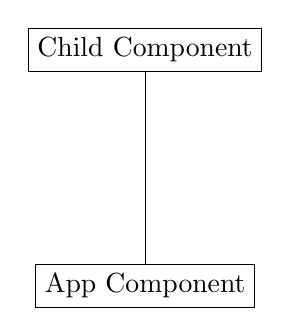
\begin{tikzpicture}[scale=3]
	\node[rectangle,draw] (App) at (0,0) {App Component};
	\node[rectangle,draw] (Child) at (0,1) {Child Component};
	% draw the line
	\draw (App) -- (Child);
\end{tikzpicture}
But with complex app architecture as shown, it gets very difficult and painful to exchange data between components. Consider if we had to pass some data from cart component to the navbar component.

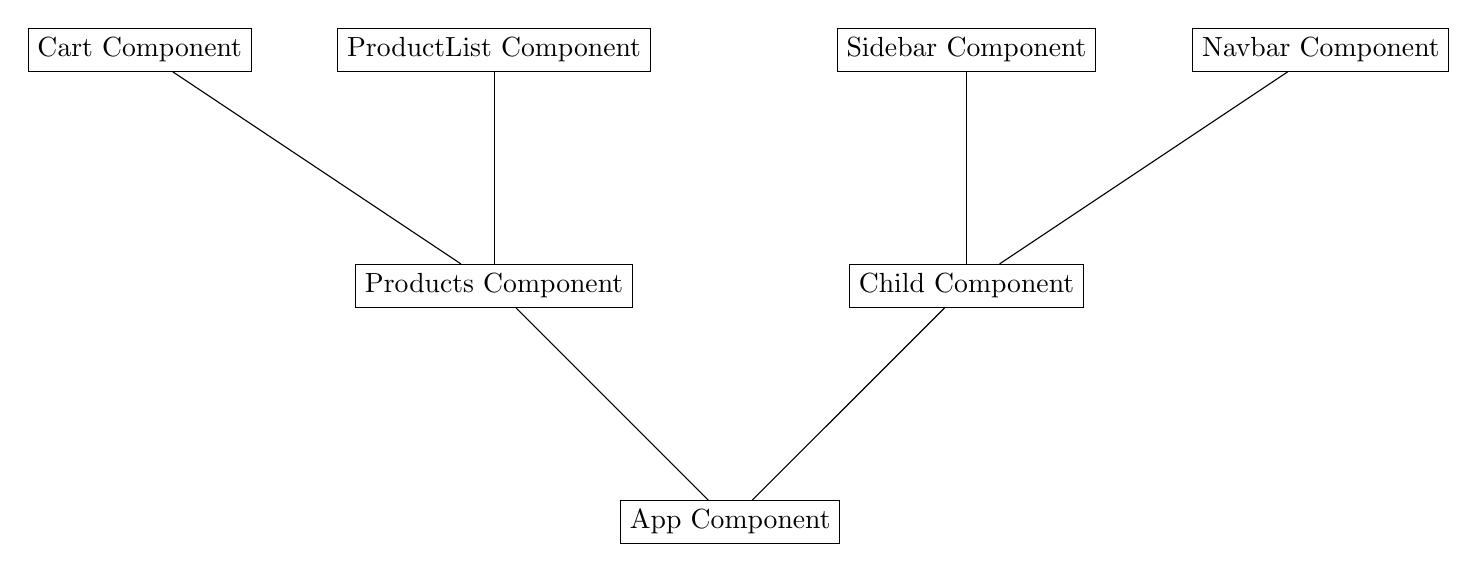
\begin{tikzpicture}[scale=3]
	\node[rectangle,draw] (App) at (0,0) {App Component};
	\node[rectangle,draw] (Home) at (1,1) {Child Component};
	\node[rectangle,draw] (Products) at (-1, 1) {Products Component};
	\node[rectangle,draw] (Navbar) at (2.5,2) {Navbar Component};
	\node[rectangle,draw] (Sidebar) at (1,2) {Sidebar Component};
	\node[rectangle,draw] (ProductList) at (-1,2) {ProductList Component};
	\node[rectangle,draw] (Cart) at (-2.5,2) {Cart Component};
	% draw the line
	\draw (App)      -- (Home);
	\draw (App)      -- (Products);
	\draw (Home)     -- (Navbar);
	\draw (Home)     -- (Sidebar);
	\draw (Products) -- (ProductList);
	\draw (Products) -- (Cart);
\end{tikzpicture}

State management is a technique that we use to handle the state of the application effectively to ensure the consistency of data across the application.
We will be using ngRx for state management in angular.

Next we will learn about ngRx in detail.
\section{ngRx}
\textbf{ngRx} stands for Angular Reactive Extensions.

It is an open source library that helps to build reactive applications using angular.
It is a great design pattern for predictable state management, which is inspired by Redux (a state management library for React).
It aims to bring reactive extensions to angular and redux like a single store for the state in an application.

Redux Patter + RxJs + Angular = ngRx

Some of the features provided by ngRx are:
\begin{itemize}
	\item{State management}
	\item{Isolation of side effects}
	\item{Router bindings}
	\item{Entity collection management}
\end{itemize}
ngRx should be used in medium/complex applications which involve a lot of user interactions and multiple data sources.

A good way to decide whether we need ngRx in our angular applications is SHARI principle of ngRx.
\begin{itemize}
	\item{Shared: state that is accessed by many components and services.}
	\item{Hydrated: state that is persisted and rehydrated from external storage.}
	\item{Available: state that needs to be available when re-entering routes.}
	\item{Retrieved: state that must be retrieved with a side-effect.}
	\item{Impacted: state that is impacted by actions from other sources}
\end{itemize}

Let's consider an event that we all are likely to be familiar with - visiting a library to borrow a few books.

Let's say, one morning you wake up and want to read some books.

Rather than buying them, you decide to visit your local library to issue them instead. While going to the library there’s just one intention or action you’ve got in mind i.e. BORROW (issue/borrow a book).

Here’s where things will get interesting, in the above scenario, there are three main tasks that are happening:

\begin{itemize}
	\item{A Library which has all the books stored for not only you, but many others.}
	\item{The Customer (you) wants to access the books in library without much hassle}
	\item{You relied on someone else (a Librarian), to smoothly and efficiently let you borrow some books. }
	\item{And definitely not to forget the Book itself}
\end{itemize}

You are being the customer of the Library, looking to borrow some books. You won't go directly to the Library's book racks and take a book on your own. Rather you need to rely upon the library system that includes a librarian to handover your required books to you. 
Thats where Redux pattern plays a role in ngRx for state management.

The previous scenario is very common, and is faced by almost all of us.

Your issued books in the library signifies your 'state' with respect to the Library. Library as institution manages everyone else's books along with managing your books specifically. For which, the Library has created different accounts (or library cards) to preserve the 'state' of each of its customers.

The library company can be thought of as ngRx as a whole. This scenario has four main actors involved: 
\begin{itemize}
	\item{Book racks: This is the only single source of books, which is being used for everyone's transactions (borrow/returning/extension etc).}
	\item{You: You are the one who want to borrow (or return) the books. The library has your existing state with it, and you are relying on the library system to get your book out of the pool of books sitting inside the library.}
	\item{A Librarian: They are the agents for the actual management of money. A librarian will validate if you have the authority and the necessary availability of books for your transaction. }
	\item{The Book: The book rack is going to have a lot of books placed. We don't need the entire book rack, rather we want only the book of our choice.}
\end{itemize}
A library transaction results in the manipulation of books or the 'state' in the Library. Hence, the librarian is the person who is responsible for changing from one 'state' to another.

Likewise, ngRx is similar to the library company. ngRx also has four main parts:
\begin{itemize}
	\item{Store - Store is the place where all the possible states of all the components of your application are stored. Store in ngRx can be understood as the book racks of a library where the books for all the customers are kept.}
	\item{Actions - Action is the one which initiates a request to change the 'state'. In our example, Action is analogous to you. As Action initiates state change, similarly, you are the one who initiates any book borrow or book return from your account.}
	\item{Reducers - These are the agents that change the state of app, in a smooth and predictable manner. Reducers are analogous to the librarian who are responsible for any borrow or return of books happening in the library.}
	\item{Selectors - When the customer borrows a book, the library does not provide the entire book rack to the customer. It just gives the required book to customer. The same job is done by the Selector in ngRx. It provides only the required states from the store.}
\end{itemize}

Hence, the main actors in ngRx for any state management are Store, Reducers, Selectors and Actions.
Next, lets see the principles of redux based on which ngRx works.
\section{Redux Principles of ngRx}
ngRx is based on the three fundamental principles of Redux:

\begin{itemize}
	\item{Single source of truth}
	\item{State is immutable}
	\item{Changes are made with pure functions}
\end{itemize}

\begin{enumerate}
	\item{Single source of truth}
		The state of complete application is stored in a single state object tree within a store. Having single store in a application makes it easy to create, debug and test. It also means components should read data from this single source and not keep their own version of the same state separately. The state of whole application is centralized and stores in a single state object. In ngRx, store is the single source of truth.
	\item{ State is immutable}
		State is immutable. The only way to change a state is by dispatching an action. Since whole application is stored in single state tree, having immutable state make sure that no views or network callbacks wrote directly to state. Instead, they dispatch an action, which have type property which indicates the  type of action being performed.
	\item{Changes are made with pure functions}
		Pure functions are those functions which do not change input value and always provide same output for same input. In Redux/ngRx, reducers are pure functions which takes previous state and an action as parameter and return new state.Since reducers are pure functions, it will never change the previous state, it will always return new state object.
\end{enumerate}
\section{ngRx Core Concepts}
Then, based on the action we create, the changes must be applied into the state available in the \textbf{ngRx Store}. To apply those changes into the state based on the action, we use Reducers.

Once the new application state is produced, we need to select the state/data from the store that are required in the components and then pass it on to them, this job of selecting the data from the store and then passing on to the components is done by a Selector.

So, In Short, we can say, A component creates an \textbf{action} based on user \textbf{events}, which then goes to the reducer, based on the action the reducer updates the \textbf{store} and then \textbf{selector} passes on the required state to the respective components.

Now, the application might not be that simple always, some user events might also involve asynchronous http calls. To manage such asynchronous operations, we use \textbf{Effects}. These \textbf{Effects} will help us invoke the required services to interact with the database and hence bring back appropriate response which will be later used to update the store.

\section{Action}
Actions are one of the main building blocks in NgRx. Actions represent unique events in ngRx based angular application and each action updates the state differently. There are many ways in which an action can be created such as:
\begin{itemize}
	\item{user interaction through clicks, mouseovers, form submissions, etc...}
	\item{external interaction through network requests,}
	\item{direct interactions with device APIs, etc..}
\end{itemize}
An action is made up of a simple interface containing a property type.

\begin{lstlisting}[caption=action.ts, language=Typescript]
	interface Action {
		type: string;
	}
\end{lstlisting}
The property type describes the action to be dispatched. The value for type property will be in the form '[Source] Event' where we use Source to specify source from where action was created. A simple of action is:


\begin{lstlisting}[caption=example-action, language=Typescript]
	{ type: '[Counter Component] Increment' }
\end{lstlisting}

We can also pass additional data (also known as payload) with the action as given below

\begin{lstlisting}[caption=example-action, language=Typescript]
	{ type: '[Login Page] Login', username: string; password: string;}
\end{lstlisting}

payload: payload is not compulsory to be passed with every action. The data type of the payload depends on the type of data that the actions needs to send to the reducer.

\subsection{Action Creators}
Actions can be created using the createAction method available from the @ngrx/store library. Following are few examples for createAction method:
\begin{lstlisting}[caption=without payload, language=Typescript]
	import { createAction } from '@ngrx/store';
	export const increment = createAction('[Counter Component] Increment');
	/* increment() returns { type: '[Counter Component] Increment'} */

\end{lstlisting}

\begin{lstlisting}[caption=with payload, language=Typescript]
	import { createAction, props } from '@ngrx/store';
	export const login = createAction(
	'[Login Component] Login',
	props<{ username: string; password: string }>()
	);
	/* login('user1', 'user1') returns {type: '[Login Component] Login', username:'user1', password:'user1' } */
\end{lstlisting}
createAction function will return a function that when called will return an object as shown before in this page. props() method helps to payload data. 

createAction just returns an action object which then must be dispatched based on any event that occurs due to user interaction. An action can be dispatched from the components using the dispatch method of store as given below:

\begin{lstlisting}[caption=example, language=Typescript]
	this.store.dispatch(increment()); /* Without Payload */
	this.store.dispatch(login("user1", "user1")); /* With Payload */
\end{lstlisting}

%https://lex.infosysapps.com/web/en/viewer/web-module/lex_auth_013031438704893952264?collectionId=lex_auth_0127668079785820163566&collectionType=Course&pathId=lex_auth_013888821194940416618
\section{Reducer}
Reducers are the pure function that handles the state of the application based on the type of the action triggered. It takes the previous state and an action as an argument and returns a new state and hence, it transitions the application from one state to another.
There are a few consistent parts of every state managed by a reducer which includes:
\begin{itemize}
	\item{An Interface or a data type to define the type of state}
	\item{It will always have two parameters i.e. initial/current state and current action}
	\item{Function to handle the state changes for the the current action}
\end{itemize}

\subsection{example}
First thing we need to do is define the type of the State using an interface as given below:
\begin{lstlisting}[caption=state.ts, language=Typescript]
	export interface State {
		counter : number;
	}
\end{lstlisting}

Once the state's type has been defined, we also need to create an initial state object of the type State.

\begin{lstlisting}[caption=initial-state.ts, language=Typescript]
	export const initialState: State = {
		counter: 0
	};
\end{lstlisting}

After defining the initial state, We need to define the reducer function that will handle the different actions.
Reducers can be created using the createReducer method available from the @ngrx/store library. Following is an example to use createReducer method:

\begin{lstlisting}[caption=counter-reducer.ts, language=Typescript]
	import { createReducer, on } from '@ngrx/store';
	import { increment, decrement, reset } from './counter.actions'; /* This file contains all the actions */
	const _counterReducer = createReducer(initialState,
			on(increment, state => { return { ...state, counter: state.counter + 1 } }),
			on(decrement, state => { return { ...state, counter: state.counter - 1 } }),
			on(reset, state => initialState),
	);
	export function counterReducer(state, action) {
			return _counterReducer(state, action);
	}
\end{lstlisting}

\textbf{Note}: The exported counterReducer function is necessary as function calls are not supported by the AOT compiler.

In the above example, counterReducer handles 3 actions: '[Counter Component] Increment', '[Counter Component] Decrement' and '[Counter Component] Reset'. Each of these actions are strongly typed and handle the state changes immutably i.e. state transition does modify the original state instead it returns a new state object using spread operator. 

When an action is dispatched, ngRx will go through all the reducers by passing the previous state and the Action till it finds a reducer to handle the action. Whether the reducer handles the action or not, is determined by the on function.

\section{Store}
Store is a container that holds the entire application’s state.
\newline
The store helps us to keep the application data in one place, and also which enables us to use the store as a single source of truth, i.e. we can reliably access the application's state from the store rather than components of the app holding their own state and passing data between then on need. This reduces the communication between the components, which helps to scale the application without adding more complexity.

To access and manipulate the global store, we must first register it within our angular application along with the reducer function that should change the state of the application. To register the global store within our application, we use \lstinline{StoreModule.forRoot()} method with a map of key-value pairs that define our state.

Let us see how to set up an application store:

We can configure the \lstinline{app.module} with \lstinline{@ngrx/store} module and reducer as follows, by importing the application reducer into the \lstinline{StoreModule}:

\begin{lstlisting}[caption=app.module.ts, language=Typescript]
	import { BrowserModule } from '@angular/platform-browser';
	import { NgModule } from '@angular/core';
	import { AppComponent } from './app.component';
	import { StoreModule } from '@ngrx/store';
	import { counterReducer } from './counter.reducer';

	@NgModule({
		declarations: [AppComponent],
		imports: [
			BrowserModule,
			StoreModule.forRoot({ count : counterReducer })
		],
		providers: [],
		bootstrap: [AppComponent],
	})
	export class AppModule {}
\end{lstlisting}

Registering states with \lstinline{StoreModule.forRoot()} ensures that the states are defined upon application startup. In general, we register root states that always need to be available to all areas of your application immediately.
We can also configure the reducers and state for lazy loaded feature modules using \lstinline{forFeature()} method.
The store also provide us with a method dispatch which is used to dispatch actions to update the state.

\subsection{Advantages of Store based application:}

The primary advantages of a store based application are:
\begin{enumerate}
	\item{Centralized and Immutable State: As all the relevant data/state is kept at a single place, it makes the tracking of issues/bugs in the applications easier.}
	\item{Performance:  As the entire state of the application is centralized, the components can access the updated data directly from there and this improves the performance of the application as the data exchange is much simpler and faster.}
	\item{Testability: Reducer functions are pure functions and they are the ones which handle all the state updates. Pure functions are also easier to test as it simply involves input in, assert against output.}
	\item{Tooling and Ecosystem: As the state is centralized and immutable, it also empowers us with better tooling. for example, ngRx developer tools, which maintain a history of all the dispatched actions and state changes done which allows time travel during development.}
\end{enumerate}

\section{Selector}
\textbf{Selectors} are pure functions used for obtaining slices of store state. \lstinline{@ngrx/store} provides a few helper functions for optimizing this selection. Selectors provide many features when selecting slices of state such as \textbf{Portability}, \textbf{Memoization}, \textbf{Composition}, \textbf{Testability} and \textbf{Type Safety}.
We can create selectors using the functions \lstinline{createSelector} or \lstinline{createFeatureSelector}.

The \lstinline{createSelector} function can be used to select only the required data for a component from all the entire state. We can pass upto 8 selector functions as parameter to \lstinline{createSelector} method for better state selection.
Lets see a simple example with a single selector function:

\begin{lstlisting}[caption=create-selector-example.ts, language=Typescript]
	import { createSelector } from '@ngrx/store';
	export interface FeatureState {
			counter: number;
	}
	export interface AppState {
			count: FeatureState;
	}
	export const selectFeature = (state: AppState) => { return state.count };
	export const selectFeatureCount = createSelector(
			selectFeature,
			(state: FeatureState) => state.counter
	);
\end{lstlisting}

Then to fetch the value of counter function in respective components, we need to use select method by passing the selector method i.e. \lstinline{selectFeatureCount} as given below:
\begin{lstlisting}[caption=use the selector created, language=Typescript]
	this.count$ = this.store.pipe(select(fromRoot.selectFeatureCount))
\end{lstlisting}

When these functions are used to create the selectors, \lstinline{@ngrx/store} keeps track of the latest arguments in which the selector function was invoked. As Selectors are pure functions, it can return the last result without re invoking the selector function, if the arguments match with the previous one. This can help in boosting the performance of the application and is also called as \textbf{Memoization}.

\section{\textbf{ngRx Counter App - Demo}}

\textbf{Problem Statement}: Create an angular app with counter component as shown using ngRx core concepts i.e. Store, Actions, Reducers and Selectors.

\begin{enumerate}
	\item{Create an angular app and install \lstinline{@ngrx/store} in the application using the below command}
		\begin{lstlisting}[language=bash]
			npm install @ngrx/store --save
	\end{lstlisting}
\item{Create \textit{app/Store/actions/counter.actions.ts} within src with the following code:}
			\begin{lstlisting}[language=Typescript,	caption=app/Store/actions/counter.actions.ts]
				import { createAction, props } from '@ngrx/store';
				export const increment = createAction('[Counter Component] Increment');
				export const decrement = createAction('[Counter Component] Decrement');
				export const multiply = createAction('[Counter Component] Multiply', props<{ multiplyBy: number }>());
				export const reset = createAction('[Counter Component] Reset');
\end{lstlisting}
\item{Create \textit{app/Store/reducers/counter.reducer.ts} within src with the following code:}
		\begin{lstlisting}[language=Typescript,	caption=app/Store/reducers/counter.reducer.ts]
			import { createReducer, on } from '@ngrx/store';
			import { increment, decrement, reset, multiply } from '../actions/counter.action';
			export const initialState = {
					counter: 0
			};
			const _counterReducer = createReducer(initialState,
					on(increment, state => { return { ...state, counter: state.counter + 1 } }),
					on(decrement, state => { return { ...state, counter: state.counter - 1 } }),
					on(multiply, (state, { multiplyBy }) => { return { ...state, counter: state.counter * multiplyBy } }),
					on(reset, state => initialState),
			);
			export function counterReducer(state, action) {
					return _counterReducer(state, action);
			}
\end{lstlisting}
\item{Create \textit{app/Store/selectors/counter.selector.ts} within src with the following code:}
		\begin{lstlisting}[language=Typescript, caption=app/Store/selectors/counter.selector.ts]
			import { createSelector } from '@ngrx/store';
			export interface FeatureState {
					counter: number;
			}
			export interface AppState {
					count: FeatureState;
			}
			export const selectFeature = (state: AppState) => { return state.count };
			export const selectFeatureCount = createSelector(
					selectFeature,
					(state: FeatureState) => state.counter
			);
\end{lstlisting}
\item{Create a component \textbf{"counter"} and add the following code to \textit{counter.component.ts}}
		\begin{lstlisting}[language=Typescript, caption=counter.component.ts]
			import { Component, OnInit } from '@angular/core';
			import { Store, select } from '@ngrx/store';
			import { Observable } from 'rxjs';
			import { increment, decrement, reset, multiply } from '../Store/actions/counter.action';
			import * as fromRoot from '../Store/selectors/counter.selector';
			@Component({
				selector: 'app-counter',
				templateUrl: './counter.component.html',
				styleUrls: ['./counter.component.css']
			})
			export class CounterComponent implements OnInit {
				count$: Observable<number>;
				constructor(private store: Store<fromRoot.AppState>) {
				}
				ngOnInit(): void {
					this.count$ = this.store.pipe(select(fromRoot.selectFeatureCount))
				}
				increment() {
					this.store.dispatch(increment());
				}
				decrement() {
					this.store.dispatch(decrement());
				}
				reset() {
					this.store.dispatch(reset());
				}
				multiplyByTwo() {
					this.store.dispatch(multiply({ multiplyBy: 2 }))
				}
				multiplyByThree() {
					this.store.dispatch(multiply({ multiplyBy: 3 }))
				}
			}
\end{lstlisting}
\item{Add the following code to \textit{counter.component.html}}
	\begin{lstlisting}[language=HTML, caption=counter.component.html]
		<div class="card shadow row col-md-6 offset-md-3 mt-5 text-center">
			<div class="card-body">
					<h3 style="font-family: cursive;">Current Count: {{ count$  | async }}</h3>
					<button class="btn btn-outline-danger mr-2" id="increment" (click)="increment()">Increment</button>
					<button class="btn btn-outline-success mr-2" id="decrement" (click)="decrement()">Decrement</button>
					<button class="btn btn-outline-dark mr-2" id="reset" (click)="reset()">Reset Counter</button>
					<button class="btn btn-outline-warning mr-2" id="multiply" (click)="multiplyByTwo()">Multiply By 2</button>
					<button class="btn btn-outline-info" id="multiply" (click)="multiplyByThree()">Multiply By 3</button>
			</div>
		</div>
\end{lstlisting}
\item{\textit{app.module.ts}}
	\begin{lstlisting}[language=Typescript, caption=app.module.ts]
		import { BrowserModule } from '@angular/platform-browser';
		import { NgModule } from '@angular/core';
		import { AppRoutingModule } from './app-routing.module';
		import { AppComponent } from './app.component';
		import { CounterComponent } from './counter/counter.component';
		import { StoreModule } from '@ngrx/store';
		import { counterReducer } from './Store/reducers/counter.reducer';
		@NgModule({
			declarations: [
				AppComponent,
				CounterComponent
			],
			imports: [
				BrowserModule,
				AppRoutingModule,
				StoreModule.forRoot({ count: counterReducer })
			],
			providers: [],
			bootstrap: [AppComponent]
		})
		export class AppModule { }
\end{lstlisting}
\end{enumerate}

\section{Meta Reducers}
\textbf{@ngrx/store} helps us to compose all the reducers together into a single reducer. Meta Reducer is a higher order reducer function that accepts reducers and returns a new reducer.

As developers, we can consider meta reducer as a hook between action $\rightarrow$ reducer pipeline and it helps pre process the action before the normal reducers are invoked.
Some of the common use cases for meta reducers are:
\begin{itemize}
	\item{Reset State once a user session terminates}
	\item{Loggers to help developers in debugging}
	\item{Rehydrating once the app restarts}
\end{itemize}

Meta reducers are the reducer functions which should be executed irrespective of the action type.

Meta reducers are very similar to the \textbf{middlewares} in redux.
\subsection{Demo}
\textbf{Problem Statement}: Log all the dispatched actions and state changes in browsers console

Update the code in \textit{app.module.ts} with the code given below in the counter-app used in previous demo:
\begin{lstlisting}[language=Typescript, caption=app.module.ts]
import { BrowserModule } from '@angular/platform-browser';
import { NgModule } from '@angular/core';
import { AppRoutingModule } from './app-routing.module';
import { AppComponent } from './app.component';
import { CounterComponent } from './counter/counter.component';
import { StoreModule, ActionReducer, MetaReducer } from '@ngrx/store';
import { counterReducer } from './Store/reducers/counter.reducer';
/* console.log all actions and state changes */
export function debug(reducer: ActionReducer<any>): ActionReducer<any> {
	return function (state, action) {
		console.log('previous state', state);
		console.log('action', action);
		let nextState = reducer(state, action);
		console.log('current state', nextState);
		return nextState;
	};
}
export const metaReducers: MetaReducer<any>[] = [debug];
@NgModule({
	declarations: [
		AppComponent,
		CounterComponent
	],
	imports: [
		BrowserModule,
		AppRoutingModule,
		StoreModule.forRoot({ count: counterReducer }, { metaReducers })
	],
	providers: [],
	bootstrap: [AppComponent]
})
export class AppModule { }
\end{lstlisting}

\textbf{Line 6:} ActionReducer and MetaReducers are imported from \textbf{@ngrx/store}. \lstinline{ActionReducer} is a function that takes an Action and a state and return another State. It is used to ensure, debug function takes a reducer function as a parameter.\\
\textbf{Line 9:} debug is a reducer function that takes a \lstinline{ActionReducer} as a parameter and returns another \lstinline{ActionReducer}. It returns another function that logs the dispatched action, state before and after the action was handled by the corresponding reducer.\\
\textbf{Line 18:} metaReducer is an array of meta-reducers to be used, in this case we are using only one i.e. debug meta-reducer.\\
\textbf{Line 27:} metaReducer has been configured to the application using \lstinline{StoreModule.forRoot()}.

\section{ngRx Dev Tools}
Store Devtools provides developer tools and instrumentation for Store.
To use ngrx devtools, we first need to install @ngrx/store-devtools:
\begin{lstlisting}[language=bash]
npm install @ngrx/store-devtools --save
\end{lstlisting}
\textbf{Setup}

Follow the given steps to configure the store devtools for chrome:
\begin{enumerate}
	\item{Add the Redux Devtools Extension to your chrome from the chrome web store.}
	\item{In app.module.ts, add the module imports using StoreDevtoolsModule.instrument as shown below:}
	\begin{lstlisting}[language=Typescript, caption=app.module.ts]
	/* Add the following import statements to the file */
import { StoreDevtoolsModule } from '@ngrx/store-devtools';
import { environment } from '../environments/environment';
/* Add the following code to imports array of AppModule */
StoreDevtoolsModule.instrument({
			maxAge: 25,
			logOnly:environment.production
		})

	\end{lstlisting}
\end{enumerate}
maxAge:25 will ensure that the last 25 state changes data is maintained in the devtools.
logOnly will connect to the devtools extension in log-only mode.By default it is false, which enables all the extension features.
The devtools has many more other \href{https://ngrx.io/guide/store-devtools/config}{options} available.
\section{Demo : NgRx/store}
Understanding the core modules of ngRx through a counter-demo
Creating action, reducer, and store

\begin{enumerate}
	\item{Create an angular application and install ngrx/store in the same folder:}
		\begin{lstlisting}[language=bash]
		npm install @ngrx/store
	\end{lstlisting}

\item{ Create \textit{app/actions/counter.actions.ts} within src as shown below:}
		\begin{lstlisting}[language=Typescript, caption=app/actions/counter.actions.ts]
		import { Action } from '@ngrx/store';
export const INCREMENT_COUNT = 'INC_COUNT';
export const DECREMENT_COUNT = 'DEC_COUNT';
export class IncrementCounter implements Action {
	readonly type = INCREMENT_COUNT;
	constructor(public payload: number) {
	}
}
export class DecrementCounter implements Action {
	readonly type = DECREMENT_COUNT;
	constructor(public payload: number) {
	}
}
export type Actions = IncrementCounter | DecrementCounter;

\end{lstlisting}
\item{ Create \textit{app/reducers/counter.reducer.ts} within src as shown below:}
		\begin{lstlisting}[language=Typescript, caption=app/reducers/counter.reducer.ts]
		import * as counterActions from './../actions/counter.actions';
const initialState = {
	counter: 10
};
export function counterReducer(state = initialState, action: counterActions.Actions) {
	switch (action.type) {
		case counterActions.INCREMENT_COUNT: {
			console.log(state);
			return {
				...state,
				counter: state.counter + action.payload
			};
		}
		case counterActions.DECREMENT_COUNT: {
			console.log('DECREMENT_COUNT');
			console.log(state);
			return {
				...state,
				counter: state.counter - action.payload
			};
		}
		default: {
			return state;
		}
	}
}
\end{lstlisting}
\item{ Create \textit{app/counter/counter.component.ts} within src as shown below:}
		\begin{lstlisting}[language=Typescript, caption=app/counter/counter.component.ts]
		import { Component, OnInit } from '@angular/core';
import { Store, select } from '@ngrx/store';
import * as counterActions from './../actions/counter.actions';
@Component({
	selector: 'app-counter',
	templateUrl: './counter.component.html',
	styleUrls: ['./counter.component.css']
})
export class CounterComponent implements OnInit {
	constructor(private store: Store<any>) { }
	count: number = 0;
	ngOnInit() {
		this.store.select('counterReducer').subscribe(
			counter => {
				console.log("sub", counter);
				if (counter) {
					this.count = counter.counter;
				}
			}
		);
	}
	onAddCount(counter?: number) {
		console.log(counter);
		this.store.dispatch(new counterActions.IncrementCounter(counter),
		);
	}
	onDecrementCount(counter?: number) {
		console.log(counter);
		this.store.dispatch(new counterActions.DecrementCounter(counter),
		);
	}
}
\end{lstlisting}
\item{Create \textit{app/counter/counter.component.html} within src as shown below:}
	\begin{lstlisting}[language=HTML, caption=app/counter/counter.component.html]
	<div style="background-color:skyblue ;width:500px;"><br/>
	<h2>&nbsp;&nbsp;Counter</h2><br/>
	<div>
			&nbsp; &nbsp;
	<button (click)="onAddCount(2)" value="click">Increment</button>
&nbsp;&nbsp;&nbsp;
	<button (click)="onDecrementCount(2)" value="click">Decrement</button>
<br/><br/>
 <h5>&nbsp;&nbsp;&nbsp;Counted: {{count}}</h5> <br/><br/>
</div>
<div style="background-color:skyblue ;width:500px;"><br/>
	<h2>&nbsp;&nbsp;Counter</h2><br/>
	<div>
			&nbsp; &nbsp;
	<button (click)="onAddCount(2)" value="click">Increment</button>
&nbsp;&nbsp;&nbsp;
	<button (click)="onDecrementCount(2)" value="click">Decrement</button>
<br/><br/>
 <h5>&nbsp;&nbsp;&nbsp;Counted: {{count}}</h5> <br/><br/>
</div>

\end{lstlisting}
\item{Create \textit{app/app.component.ts} within src as shown below:}
	\begin{lstlisting}[language=Typescript, caption=app/app.component.ts]
	import { Component } from '@angular/core';
@Component({
	selector: 'app-root',
	templateUrl: `<div >
	<h4>
	Counter demo which explains NgRx modules
	</h4>
</div>
<app-counter></app-counter>`,
	styleUrls: ['./app.component.css']
})
export class AppComponent {
	title = 'ngrx demo app';
}

\end{lstlisting}
\item{ Create \textit{app/app.module.ts} within src as shown below:}
	\begin{lstlisting}[language=Typescript, caption=app/app.module.ts]
	import { BrowserModule } from '@angular/platform-browser';
import { NgModule } from '@angular/core';
import { AppComponent } from './app.component';
import { CounterComponent } from './counter/counter.component';
import { counterReducer } from './reducers/counter.reducer';
import { StoreModule } from '@ngrx/store';
@NgModule({
	declarations: [
		AppComponent,
		CounterComponent
	],
	imports: [
		BrowserModule,
		StoreModule.forRoot({counterReducer: counterReducer})
	],
	providers: [],
	bootstrap: [AppComponent]
})
export class AppModule { }
\end{lstlisting}

\end{enumerate}

\section{ngRx Effects}
In any service based application which interacts with a database server, component is the one which interacts with external resources directly through services. So, the component is responsible to manage the view dynamically as well as interacting with external sources.

Effects help us handle this more efficiently. Effects provide us a way to interact with the services and isolate them from the components.
Effects are an RxjS powered side effect model for Store. Effects uses streams and provide us with new sources of action to handle the state based on external interactions such as long running tasks which produce multiple events, web-socket messages and network requests to fetch, add or modify data.
The use of Effects becomes much more important in larger applications as they may have multiple sources of data with multiple services required to fetch those data

Features of Effects
\begin{itemize}
	\item{It helps to have more pure components that can select the state from the store and dispatch actions, by isolating the side effects.}
	\item{Effects are long running services which listens to every action dispatched.}
	\item{Effects use RxJS operators to filter the actions based on the type of action.}
	\item{Effects can handle synchronous as well as asynchronous tasks and return a new action.}
\end{itemize}

To use ngRx Effects in our angular applications to perform the side effects, we need to install it using the below command:
\begin{lstlisting}[language=bash]
npm install @ngrx/effects --save
\end{lstlisting}
\subsection{Writing ngRx Effects}
We can use Effects to isolate the side effects/external interactions from the components by creating a Effect class which listens to events and performs taskst.
Effect class is an injectable service class and has the following distinct parts:
\begin{itemize}
	\item{An injectable Actions service which provides an observable of all the dispatched actions after the latest state changes.}
		\begin{lstlisting}[language=Typescript, caption=product-effects.ts]
		/* Example */
import { Injectable } from '@angular/core';
import { Actions } from '@ngrx/effects';
@Injectable()
export class ProductEffects {
	constructor(private actions$: Actions) { }
}
	\end{lstlisting}
\item{Metadata is attached to the observable of dispatched actions using \lstinline{createEffect} function of @ngrx/effects. The \lstinline{createEffect} function registers the streams that are subscribed to the store. Any action returned from the effect stream is then dispatched back to the Store.}
		\begin{lstlisting}[language=Typescript, caption=product-effects.ts]
		/* Example */
import { Injectable } from '@angular/core';
import { Actions, createEffect } from '@ngrx/effects';
@Injectable()
export class ProductEffects {
		constructor(private actions$: Actions) { }
		loadProducts$ = createEffect(() => this.actions$.pipe());
}
\end{lstlisting}
\item{Actions are filtered using the ngRx effects pipeable ofType operator. It takes one or more action types as argument to filter those on which it needs to act upon.}
		\begin{lstlisting}[language=Typescript, caption=product-effects.ts]
		/* Example */
import { Injectable } from '@angular/core';
import { Actions, createEffect, ofType } from '@ngrx/effects';
@Injectable()
export class ProductEffects {
		constructor(private actions$: Actions, private productService: ProductService) { }
		loadProducts$ = createEffect(() => this.actions$.pipe(
				ofType('[ProductList Component] GET_ALL_PRODUCTS')
		));
}
\end{lstlisting}
\item{Effects are subscribed to the Store observable and Services are injected into the effects to interact with the external API's.}
		\begin{lstlisting}[language=Typescript, caption=product-effects.ts]
		import { Injectable } from '@angular/core';
import { Actions, createEffect, ofType } from '@ngrx/effects';
import { of } from 'rxjs';
import { ProductService } from '../../product-list/product.service';
import { map, mergeMap, catchError } from 'rxjs/operators';
@Injectable()
export class ProductEffects {
		constructor(private actions$: Actions, private productService: ProductService) { }
		loadProducts$ = createEffect(() => this.actions$.pipe(
				ofType('[ProductList Component] GET_ALL_PRODUCTS'),
				mergeMap(() => this.productService.getAllProducts()
						.pipe(
								map(products => ({ type: '[ProductList Component] GET_ALL_PRODUCTS SUCCESS', allProducts: products })),
								catchError(() => of({ type: '[ProductList Component] GET_ALL_PRODUCTS ERROR', errorMessage: 'No Products Found' }))
						),
				),
		)
		);
}
\end{lstlisting}
\end{itemize}

\subsubsection*{The flow Explanations:}
\begin{itemize}
	\item{The \lstinline{loadProducts$} effect is listening for all dispatched actions through the Actions stream, but is only interested in the '[ProductList Component] GET\_ALL\_PRODUCTS' event using the \lstinline{ofType} operator.}
	\item{The stream of actions is then flattened and mapped into a new observable using the \lstinline{mergeMap} operator.}
	\item{The \lstinline{productService#getAllProducts()} method returns an observable that maps the products to a new action on success, and currently returns an empty observable if an error occurs.}
	\item{The action is dispatched to the Store where it can be handled by reducers when a state change is needed.}
	\item{It's also important to handle errors when dealing with observable streams so that the effects continue running.}
\end{itemize}

\subsubsection*{Angular App flow with ngRx Effects} 
\begin{figure}[h]
	\centerline{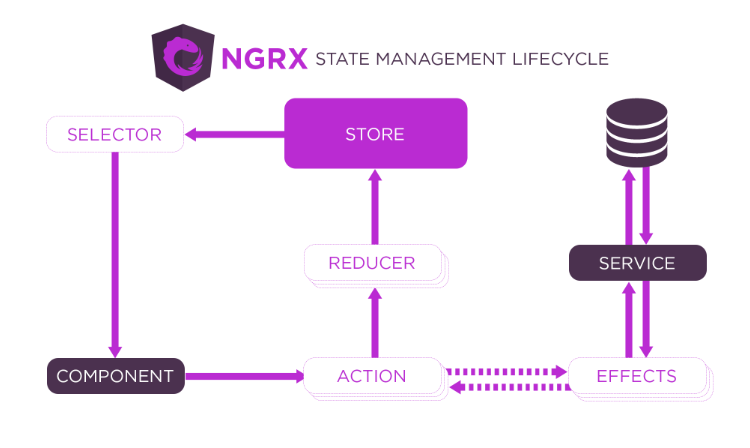
\includegraphics{ngrxflowdiagram.png}}
	\caption{Angular App flow with ngRx Effects}
	\label{Angular App flow with ngRx Effects}
\end{figure}

\begin{enumerate}
	\item{Component C Dispatches an action A.}
	\item{The action A invokes an Effect E.}
	\item{The Effect E then invokes a service Srv to interact with the database. After service call the Effect E again returns an action, either A1 or A2 depending upon service call success or error.}
	\item{A1/A2 should not be the same as A (otherwise, this will lead to infinite loop).}
	\item{These actions A1/A2 then go to the reducer R and update the store S.}
	\item{Once the store S has been updated, the component C can fetch the value using a Selector SS.}
\end{enumerate}

\subsection{ngRx Effects - Demo}
\subsubsection*{Problem Statement: Create a component product-list that uses ngRx effects to make API call for loading the list of products is success case and displays error message is if data not found}
To achieve the above requirement, Follow the below steps:

\begin{enumerate}

	\item{Create an angular app and install @ngrx/effects in the angular application:}
		\begin{lstlisting}[language=bash]
			npm install @ngrx/effects --save
	\end{lstlisting}

\item{Define a model class for the Products data in the file \textit{product-list/products.ts}:}
		\begin{lstlisting}[caption=product-list/products.ts, language=Typescript]
			export class Product {
				id: number=0;
				productName: string="";
				productPrice: number=0;
				productImg: string="";
				productBrand: string="";
			}
\end{lstlisting}

\item{Define the actions for handling both success and error cases of API calls in the file \textit{Store/actions/products.actions.ts}:}
		\begin{lstlisting}[language=Typescript, caption=Store/actions/products.actions.ts]
			import { createAction, props } from '@ngrx/store';
			import { Product } from '../../product-list/products';
			export const getAllProducts = createAction('[ProductList Component] GET_ALL_PRODUCTS')
			export const getAllProductsAPISuccess = createAction('[ProductList Component] GET_ALL_PRODUCTS SUCCESS', props<{ allProducts: Product[] }>())
			export const getAllProductsAPIError = createAction('[ProductList Component] GET_ALL_PRODUCTS ERROR', props<{ errorMessage: String }>())
		\end{lstlisting}	
	\lstinline{getAllProducts} is the action to be dispatched on load of product-list component, whereas \lstinline{getAllProductsAPISuccess} and \lstinline{getAllProductsAPIError} are the actions dispatched by the Effect once it completes the API/service call with success or error response
\item{Define the \textbf{Initial state} for the application in the file \textit{Store/states/products.store.ts}:}
		\begin{lstlisting}[caption=Store/states/products.store.ts, language=Typescript]
			export const initialProductState = {
				allProducts: [],
				errorMessage: ""
			}
\end{lstlisting}
allProducts is an array that will store an array of product objects fetched from service call whereas errorMessage will store the error response in case the service call does not return the required data.
\item{Define the reducer for handling both success and error cases of API calls in the file \textit{Store/reducers/products.reducer.ts}:}
		\begin{lstlisting}[language=Typescript, caption=Store/reducers/products.reducer.ts]
			import { createReducer, on } from '@ngrx/store';
			import { getAllProducts, getAllProductsAPISuccess, getAllProductsAPIError } from '../actions/products.actions';
			import { initialProductState } from '../states/products.store';
			const _productReducer = createReducer(initialProductState,
			on(getAllProducts, (state) => state),
			on(getAllProductsAPISuccess, (state:any, { allProducts }) => { return { ...state, allProducts: allProducts, errorMessage: "" } }),
			on(getAllProductsAPIError, (state:any, { errorMessage }) => { return { ...state, errorMessage: errorMessage, allProducts: [] } })
			);
			export function productReducer(state:any, action:any) {
				return _productReducer(state, action);
			}
\end{lstlisting}
productReducer is the reducer function that handles actions dispatched by the components as well as the effects after making the API calls
\item{Define the selectors in the file \textit{Store/selector/products.selector.ts} to ensure the component gets only the required data:}
		\begin{lstlisting}[caption=Store/selector/products.selector.ts, language=Typescript]
			import { createSelector } from '@ngrx/store';
			import { Product } from '../../product-list/products';
			export interface FeatureState {
				allProducts: Product[];
				errorMessage: String;
			}
			export interface AppState {
				products: FeatureState; 
			}
			export const selectFeature = (state: AppState) => { return state.products };
			export const selectError = (state: AppState) => { return state.products };
			export const selectFeatureProduct = createSelector(
			selectFeature,
			(state: FeatureState) => state.allProducts
			);
			export const selectFeatureError = createSelector(
			selectError,
			(state: FeatureState) => state.errorMessage
			);
\end{lstlisting}
FeatureState defines the structure of the data stored in the store object 
selectFeatureProduct will return the products array from the global array whereas selectFeatureError will return the errorMessage set by the reducer

\item{Create the Effects that invokes the appropriate service method to fetch all the products from server:}
		\begin{lstlisting}[caption=product-effects.ts, language=Typescript]
			import { Injectable } from '@angular/core';
			import { Actions, createEffect, ofType } from '@ngrx/effects';
			import { ProductService } from '../../product-list/product.service';
			import { map, mergeMap, catchError } from 'rxjs/operators';
			@Injectable()
			export class ProductEffects {
				constructor(private actions$: Actions, private productService: ProductService) { }
				loadProducts$ = createEffect(() => this.actions$.pipe(
				ofType('[ProductList Component] GET_ALL_PRODUCTS'),
				mergeMap(() => this.productService.getAllProducts()
				.pipe(
				map(products => ({ type: '[ProductList Component] GET_ALL_PRODUCTS SUCCESS', allProducts: products })),
				catchError(() => of({ type: '[ProductList Component] GET_ALL_PRODUCTS ERROR', errorMessage: 'No Products Found' }))
				))));
			}
\end{lstlisting}
createEffect is the method used to define an Effect, as discussed previously.

\item{Create a Service product with the following code to fetch all the products from the server:}
		\begin{lstlisting}[language=Typescript, caption=product.service.ts]
			import { Injectable } from '@angular/core';
			import { HttpClient } from '@angular/common/http';
			import { Observable } from 'rxjs';
			import { Product } from './products';
			@Injectable({
				providedIn: 'root'
			})
			export class ProductService {
				constructor(private http: HttpClient) { }
				getAllProducts(): Observable<Product[]> {
					return this.http.get<Product[]>("http://localhost:4000/products");
				}
			}
\end{lstlisting}
\lstinline{getAllProducts()} is a service method which makes an API call to fetch all the products data from the service

\item{Create a product-list component and add the following code to dispatch an action to fetch all the products on load of the component:}
		\begin{lstlisting}[caption=product-list.component.ts, language=Typescript]
			import { Component, OnInit } from '@angular/core';
			import { Product } from './products';
			import { Store, select } from '@ngrx/store';
			import { Observable } from 'rxjs';
			import * as fromRoot from '../Store/selector/products.selector';
			@Component({
				selector: 'app-product-list',
				templateUrl: './product-list.component.html',
				styleUrls: ['./product-list.component.css']
			})
			export class ProductListComponent implements OnInit {
				constructor(private store: Store<fromRoot.AppState>) { }
				products$: Observable<Product[]> = this.store.pipe(select(fromRoot.selectFeatureProduct))
				errorMessage$: Observable<String> = this.store.pipe(select(fromRoot.selectFeatureError))

				ngOnInit(): void {
					this.store.dispatch({ type: '[ProductList Component] GET_ALL_PRODUCTS' });
				}
			}
\end{lstlisting}
\lstinline{products$} is the property that stores the products array fetched from the global store. \lstinline{errorMessage$} is the property that stores the error message fetched from the global store. An action of type '[ProductList Component] GET\_ALL\_PRODUCTS' is dispatched on load of component using \lstinline{ngOnInit()} method.

\item{Add the following code to \textit{product-list.component.html} file:}
		\begin{lstlisting}[language=HTML, caption=product-list.component.html]
			<div class="row mt-4 text-center" style="font-family: cursive;">
			<div class="col-md-3" *ngFor="let product of products$ | async; let i = index">
			<div class="card shadow">
			<img src="{{product.productImg}}" alt="{{product.productName}}">
			<div class="card-body">
			<h5>{{product.productName}}</h5>
			<h6>Brand: {{product.productBrand}}</h6>
			<h6 class="text text-success">Price: {{product.productPrice | currency:'INR'}}</h6>
			</div>
			</div>
			</div>
			<span *ngIf="errorMessage$">{{errorMessage$ | async}}</span>
			</div>

\end{lstlisting}
asyc pipe is used for both products$ and errorMessage$ as it unwraps a value from an asynchronous primitive

\item{Configure the effects in \textit{app.module.ts} file:}
		\begin{lstlisting}[caption=app.module.ts, language=Typescript]
			import { BrowserModule } from '@angular/platform-browser';
			import { NgModule } from '@angular/core';
			import { AppRoutingModule } from './app-routing.module';
			import { AppComponent } from './app.component';
			import { ProductListComponent } from './product-list/product-list.component';
			import { HttpClientModule } from '@angular/common/http';
			import { StoreModule, ActionReducer, MetaReducer } from '@ngrx/store';
			import { productReducer } from './Store/reducers/products.reducer';
			import { EffectsModule } from '@ngrx/effects';
			import { ProductEffects } from './Store/effects/products.effects';
			export function debug(reducer: ActionReducer<any>): ActionReducer<any> {
				return function (state, action) {
					console.log('previous state', state);
					console.log('action', action);
					let nextState = reducer(state, action);
					console.log('current state', nextState);
					return nextState;
				};
			}
			export const metaReducers: MetaReducer<any>[] = [debug];
			@NgModule({
				declarations: [
				AppComponent,
				ProductListComponent
				],
				imports: [
				BrowserModule,
				AppRoutingModule,
				HttpClientModule,
				StoreModule.forRoot({ products: productReducer }, { metaReducers }),
				EffectsModule.forRoot([ProductEffects])
				],
				providers: [],
				bootstrap: [AppComponent]
			})
			export class AppModule { }

\end{lstlisting}
\lstinline{EffectsModule.forRoot()} takes an array of effects to be used in the angular application to make API calls
\item{ Define the routes in \textit{app-routing.module.ts} and load the product-list component by adding router-outlet in \textit{app.component.html}:}
		\begin{lstlisting}[caption=app-routing.module.ts, language=Typescript]
			const routes: Routes = [
			{ path: '', redirectTo: 'products', pathMatch: 'full' },
			{ path: 'products', component: ProductListComponent }
			];
\end{lstlisting}
\item{To access the server and fetch the data from the server, follow the below steps: [This is just for demonstration purpose, you can use any other server such as express web service as well, in that case below steps are not required to be followed]}
	\begin{itemize}
		\item{Install json-server globally and locally:}
				\begin{lstlisting}[language=bash]
					npm install json-server -g
					npm install json-server --save
		\end{lstlisting}
	\item{Create a \textit{db.json} file in project root folder and and add the following data:}
				\begin{lstlisting}[language=json, caption=db.json]
					{
						"products": [
						{
							"id": 1001,
							"productName":"iPhone 7s",
							"productPrice":39999,
							"productImg":"iphone.jpg",
							"productBrand":"Apple"
						},
						{
							"id": 1002,
							"productName":"Nokia 8",
							"productPrice":24499,
							"productImg":"nokiasmartphone.png",
							"productBrand":"Nokia"
						},
						{
							"id": 1003,
							"productName":"Redmi Note 8 Pro",
							"productPrice":39999,
							"productImg":"redminote8.PNG",
							"productBrand":"Xiaomi"
						},
						{
							"id": 1004,
							"productName":"Samsung Galaxy s10",
							"productPrice":39999,
							"productImg":"samsunggalaxy.jpg",
							"productBrand":"Samsung"
						}
						]
					}

	\end{lstlisting}
\item{Run the json-server}
				\begin{lstlisting}[language=bash]
					json-server --watch db.json --port 4000
\end{lstlisting}
\end{itemize}
\end{enumerate}

\chapter{Single Sign On using Angular}
\section{}
\subsection*{Single Sign-On}
When you log in to G-mail, you automatically gain access to you-tube, Google drive, Google photos, and other Google applications. Have you ever wondered how this is happening?
This is done by Single Sign On.

\subsection*{What is Single Sign-On(SSO)?}
With Single Sign-On, the user can log in to multiple services with a one-time login.
\begin{figure}[h]
	\centerline{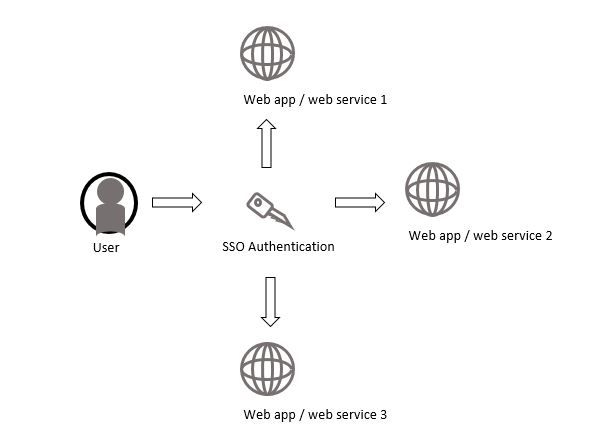
\includegraphics{newwhatissso.jpg}}
	\caption{SSO Example}
	\label{SSO Example}
\end{figure}
SSO will get the login credentials from directory server as Authentication and provides access to multiple applications by passing the authentication token to configured applications. Thus we can avoid the problem of maintaining the username and password for each site separately in their servers.
This will also help the users to get access to the different application, without maintaining separate username and password for each application.
The typical logic flow of an web application/ service with Single Sign-On will be as follows
\begin{figure}[h]
	\centerline{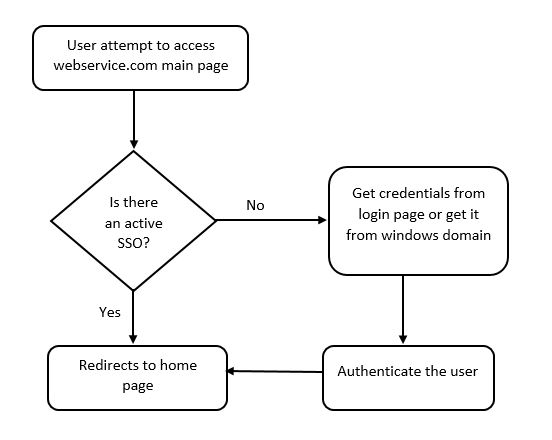
\includegraphics{SSOFlowChart1.jpg}}
	\caption{Logic flow of an web application/service with Single Sign-On}
	\label{Logic flow of an web application/service with Single Sign-On}
\end{figure}

\subsection*{SSO using Node-SSPI}
\subsubsection*{Why we need Single Sign-On(SSO)?}
\begin{itemize}
	\item{Using SSO we can eliminate the time spent on entering the user name and password for each site}
	\item{No need to remember the password for different applications}
	\item{As the SSO will get the credentials from the domain server, we can reduce the problem of storing the password in separate servers, invalid credentials, password reset issues.}
	\item{Minimize the fraudulent attempt to obtain the user name, password and some other sensitive information.}
\end{itemize}

\subsubsection*{How Single Sign-On works?}
Let us first understand how does an application work without SSO.
Normally when you want to access some web app/service, the authentication process will be as follows.

\subsubsection*{Without SSO:}
\begin{figure}[h]
	\centerline{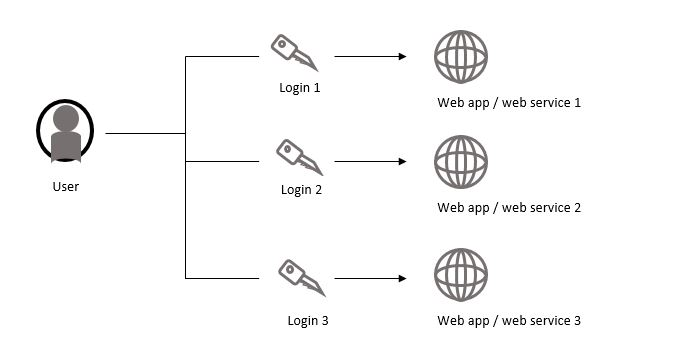
\includegraphics{newwithoutsso.jpg}}
	\caption{Without SSO}
	\label{Without SSO}
\end{figure}

\begin{itemize}
	\item{When a user enters a website, first it will check whether the user is already logged in}
	\item{If the user is logged in, it will take him/her to the home page else it will redirect to the login page.}
	\item{User has to enter his/her username and password to the website. After authentication, the user will be redirected to the login or home page}
\end{itemize}

If we do the same with the single sign-on, the steps will be like :

\subsubsection*{With SSO:}
\begin{figure}[h]
	\centerline{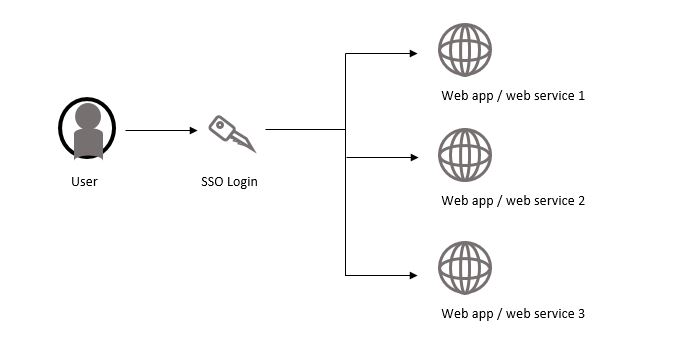
\includegraphics{newwithsso.jpg}}
	\caption{With SSO}
	\label{With SSO}
\end{figure}

\begin{itemize}
	\item{When a user enters a website, first it will check whether you are already authenticated by the SSO}
	\item{If yes, then it will take the user to the website’s home page else it will redirect him to the login page to enter username and password}
\end{itemize}
Now the user can access all the sites associated with the company without entering the username and password again.
Single Sign-On can be implemented using various platforms.
One such Platform is using Node-SSPI
\subsubsection*{Node-SSPI}
For the server side, we are using node-SSPI for authentication.
\begin{itemize}
	\item{It stands for the Security Support Provider Interface.}
	\item{NodeSSPI is modeled to perform Windows authentication through native Windows SSPI}
	\item{After successful authentication, NodeSSPI can optionally retrieve a list of groups the user belongs to, facilitating to perform authorization.}
	\item{Node.js is customizable through JavaScript which offers much more flexibility.}
\end{itemize}
\section{Demo to fetch the username - Node}
Create an Angular application that renders the username of the logged-in user.
\begin{itemize}
	\item{Create a new Express application and run the below command to install sspi package.}
	\begin{lstlisting}[language=bash]
		npm install node-expose-sspi
	\end{lstlisting}
\item{Copy the below code in your \textit{app.js} file}
		\begin{lstlisting}[language=Typescript, caption=app.js]
const express = require('express');
const { sso } = require('node-expose-sspi');
const cors = require('cors')
const bodyParser= require('body-parser')
const app = express();
const corsOptions = {
		origin: ['http://localhost:4200'],
		optionsSuccessStatus: 200,
		credentials: true
}
app.use(bodyParser.urlencoded({ extended: true }))
app.use("/", cors(corsOptions))
app.use(sso.auth());
app.use((req, res, next) => {
		res.json({
				sso: req.sso,
		});
});
app.listen(3000, () => console.log('Server started on port 3000'));
\end{lstlisting}
\item{Run the command to start the Webservice}
	\begin{lstlisting}[language=bash]
	node app.js
\end{lstlisting}
\end{itemize}
Once this is done, you can hit the URL \url{http://localhost:3000/} in browser, this will display all the available data related to the client.
We have now created the backend application, next let us understand the series of step required for using or presenting this data in the front end angular application.

\subsubsection*{Demo to fetch the username - Angular}
Follow the below steps to create your front-end application.
Step4: Create your angular application.
\begin{lstlisting}[language=bash]
ng new sso-app-ui
\end{lstlisting}
\begin{lstlisting}[caption=app.component.html, language=HTML]
<div class="container-fluid"
		*ngIf="successmessage && employeeId && location && name && emailId && department && mobileNo; else nodata">
		<div class="row mb-3 mt-2">
				<div class="col-md-6 offset-md-3">
						<div class="card shadow">
								<div class="card-header">
										<h2 class="text text-center">Hi {{successmessage}}!!</h2>
								</div>
								<div class="card-body">
										<table class="table table-hover">
												<tbody>
														<tr>
																<th>Employee Id</th>
																<td>{{employeeId}}</td>
														</tr>
														<tr>
																<th>Name</th>
																<td>{{name}}</td>
														</tr>
														<tr>
																<th>Email Id</th>
																<td>{{emailId}}</td>
														</tr>
														<tr>
																<th>Mobile Number</th>
																<td>{{mobileNo}}</td>
														</tr>
														<tr>
																<th>Location</th>
																<td>{{location}}</td>
														</tr>
														<tr>
																<th>Department</th>
																<td>{{department}}</td>
														</tr>
												</tbody>
										</table>
								</div>
						</div>
				</div>
		</div>
</div>
<ng-template #nodata>
		<div class="text text-center mt-5">
				<h2>Please wait while we prepare your profile</h2>
				<div class="spinner-border"></div>
		</div>
</ng-template>
	\end{lstlisting}

\begin{lstlisting}[caption=app.service.ts, language=Typescript]
import { Injectable } from '@angular/core';
import { HttpClient, HttpHeaders } from '@angular/common/http';
const httpOptions = {
	headers: new HttpHeaders({ 'Content-Type': 'application/json' })
};
@Injectable({
	providedIn: 'root'
})
export class AppService {
	constructor(private http: HttpClient) { }
	getData() {
		return this.http.get('http://localhost:3000/', { withCredentials: true })
	}
}
\end{lstlisting}

\begin{lstlisting}[caption=app.component.ts, language=Typescript]
import { Component } from '@angular/core';
import { AppService } from './app.service';
@Component({
	selector: 'app-root',
	templateUrl: './app.component.html',
	styleUrls: ['./app.component.css']
})
export class AppComponent {
	title = 'sso-demo-ui';
	successmessage: any;
	errorMessage: any;
	name: any;
	emailId: any;
	department: any;
	employeeId:any;
	location: any;
	mobileNo: any;
	constructor(private appservice: AppService) {
	}
	ngOnInit() {
		this.appservice.getData().subscribe(
			(success) => {
				console.log(success, typeof success);
				let data : any = success;
				this.successmessage= data.sso.user.name;
				this.name = data['sso']['user']['displayName'];
				this.emailId=data['sso']['user']['domain'];
				 this.department=data['sso']['user']['adUser']['department'];
				this.employeeId=data['sso']['user']['adUser']['company'];
				this.location=data['sso']['user']['adUser']['l'];
				this.mobileNo= data['sso']['user']['adUser']['mobile'];

				console.log(this.successmessage, typeof this.successmessage);
			},
			(err) => {
				console.log(err);
				this.errorMessage = err.error.message;
			}
		)
	}
}
\end{lstlisting}

\begin{lstlisting}[caption=app.module.ts, language=Typescript]
import { BrowserModule } from '@angular/platform-browser';
import { NgModule } from '@angular/core';
import { HttpClientModule } from '@angular/common/http';
import { AppComponent } from './app.component';
@NgModule({
	declarations: [
		AppComponent,
	],
	imports: [
		BrowserModule,
		HttpClientModule
	],
	providers: [],
	bootstrap: [AppComponent]
})
export class AppModule { }
\end{lstlisting}


\begin{lstlisting}[language=bash]
ng serve --open
\end{lstlisting}
\begin{figure}[h]
	\centerline{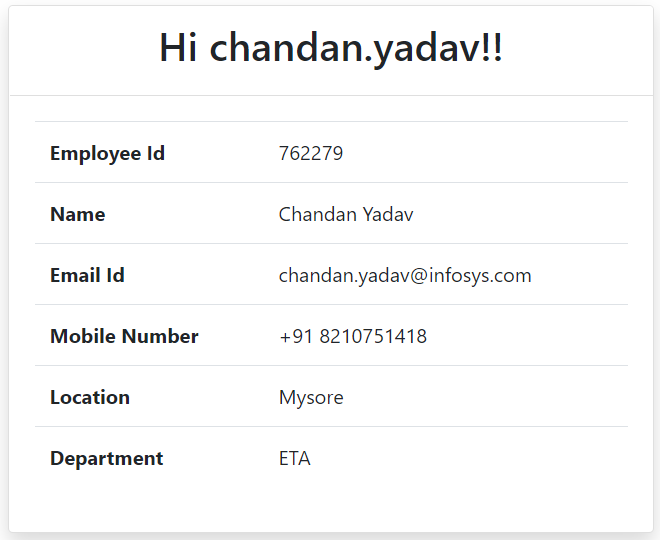
\includegraphics{ssodemooutput1619097797471.png}}
	\caption{Demo Image}
	\label{Demo Image}
\end{figure}

From this demo, we have learnt how to fetch the various details of a loggin in user. Similarly, other frontend applications can get the user logged in without asking for credentials by using the node-expose-sspi.

\section{Need for OAuth}
In most websites, we find an option to login using social networking accounts like Facebook, Twitter, Google, LinkedIn, etc. This makes login easy as we dont have to create multiple accounts in multiple web pages and facing the problem of remembering all the usernames and passwords. So how does this work?
Consider the below illustration:
\begin{figure}[h]
	\centerline{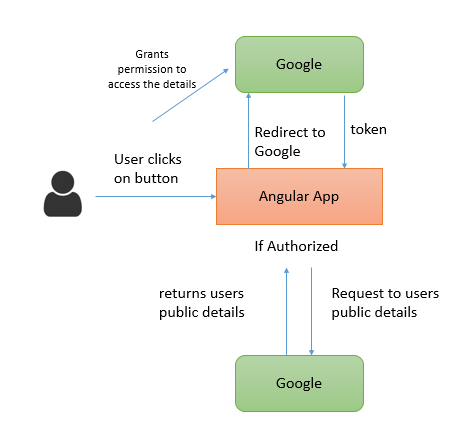
\includegraphics{oAuth.png}}
	\caption{OAuth Example Flow}
	\label{OAuth Example Flow}
\end{figure}

\begin{itemize}
	\item{The User clicks on a button in our Angular App.}
	\item{The Angular app will now redirect the user to the Google sign in page.}
	\item{The user provides his credentials in the google sign-in page ( not in our angular app ). }
	\item{By signing in, he gives permissions to our Angular app to access the users public profile data.}
	\item{When the user has thus authorized Google to allow our app to access his details.}
\end{itemize}

OAuth ( Open Authorization ) is a standard which can allow one app to authorize another app to use its details. It is basically an Authorization standard and not an authentication standard. In our example, we use Google to both authenticate and authorize the user. There are several steps in involved in creating OAuth capabilities in our Angular app. Let us look at them in the coming pages.

\subsection{Steps in OAuth}
The various steps in enabling our app with OAuth capabilities are:
\begin{enumerate}
	\item{Create a Google account}
	\item{Register our App in Google and generate Client token.}
	\item{Install an OAuth library in Angular app}
	\item{Use the client token in the Angular app}
	\item{Invoke the libraries API to contact Google and handle the response.}
\end{enumerate}
Assuming you already know how to create a Google account, let us take a look at how to register our app in \href{https://console.cloud.google.com/}{Google Cloud Platform}.
Once we have registered an app in Google, we have to use the generated tokens in the angular app. For this discussion, we will be using the \textit{angularx-social-login} node module.
The steps are:
\begin{itemize}
	\item{\lstinline{npm install angularx-social-login --save}}
	\item{Modify specific parts of the \textit{app.module.ts} as shown below:}
		\begin{lstlisting}[language=Typescript, caption=app.module.ts]
		import { SocialLoginModule } from 'angularx-social-login';
import { AuthServiceConfig, GoogleLoginProvider } from 'angularx-social-login';
const config = new AuthServiceConfig([
	{
		id: GoogleLoginProvider.PROVIDER_ID,
		provider: new GoogleLoginProvider('<Your client ID generated by Google>')
	},
	imports: [
		BrowserModule,
		FormsModule,
		HttpModule,
		SocialLoginModule
	],
	providers: [
		{
			provide: AuthServiceConfig,
			useFactory: provideConfig
		}
	]
		\end{lstlisting}

	\item{Create a new component to display the login button and user details as shown below:}
		\begin{lstlisting}[language=HTML, caption=HTML]
		<div *ngIf="user" class="card text-center">
		<h6 class="card-header">
			 Logged In with Google
		</h6>
		<div class="card-block"></div>
		<img class="card-img-top img-responsive photo" src="{{ user.photoUrl }}">
		<div class="card-block">
			<h4 class="card-title">{{ user.name }}</h4>
			<p class="card-text">{{ user.email }}</p>
		</div>
		<div class="card-block">
			<button class="btn btn-danger" (click)="signOut()">Sign out</button>
		</div>
	</div>
	\end{lstlisting}

		\begin{lstlisting}[language=Typescript, caption=TS]
		user: SocialUser;
	constructor(private authService: AuthService) { }
	ngOnInit() {
		this.authService.authState.subscribe((user) => {
			this.user = user;
			console.log(user);
		});
	}
	signInWithGoogle(): void {
		this.authService.signIn(GoogleLoginProvider.PROVIDER_ID).then(x => console.log(x));
 Click here to download zip folder :Steps in Angular App-Oauth.zip
		\end{lstlisting}
\end{itemize}
\chapter{Angular Security}
Angular provides built-in security protection for common web application vulnerabilities like XSS, CSRF, etc. Let us see how Angular handles them.
\subsection*{Cross-site scripting (XSS):}
The cross-site scripting attack happens when malicious code is injected into the webpage. This malicious code can steal or modify the user’s data and impersonate the user. In the OWASP Top 10 2021, Cross-Site-Scripting is also included under the Injection category and is one of the most common attacks on web applications.

To prevent XSS attacks, malicious code should be sanitized before entering the DOM. Sanitization is all about converting untrusted values to a safe format that can be inserted into DOM. Angular handles this by treating all values as untrusted by default. Angular escapes the untrusted values whenever malicious data is entered into DOM using interpolation or binding. 

DomSanitizer class of Angular helps to sanitize the values and helps to prevent XSS attacks.
\subsection*{Server-side XSS:}
XSS attacks can also happen to server-side code, which enables attackers to exploit the complete application. HTML rendered from the server is vulnerable to injection attacks which give attackers complete control of your Angular application. To mitigate this, use a templating language that automatically escapes the untrusted values and helps to block the attacks. Angular templates generated by templating language on the server side create template injection vulnerabilities and pose a higher risk.
\subsection*{CSRF and XSSI:}
Angular has built-in support, which helps in preventing vulnerabilities like cross-site request forgery (CSRF or XSRF) and cross-site script inclusion (XSSI). Although both are mitigated primarily on the server side, Angular provides the HttpClient class, making the client-side integration easier and simpler.
You can add another layer of protection to the Angular application by setting Security Policy (CSP) header and AOT template compiler.
\subsection*{Content Security Policy}
It is an HTTP response header that helps mitigate numerous content injection attacks. It provides different directives that can be used to restrict the content loaded into a web application. It provides directives like style-src, script-src, etc.
The minimal policy required for the Angular project is:
default-src 'self'; style-src 'self' 'unsafe-inline';
Angular itself requires these settings to function correctly.
\begin{itemize}
	\item{default-src is a fallback for other resource types when they are not configured}
	\item{style-src directive restricts loading styles from invalid resources}
	\item{script-src directive restricts loading scripts from invalid resources.}
\end{itemize}
Consider the below policy:
Content-Security-Policy: default-src 'self' 
Setting the value of the "default-src" directive to "self" indicates that only the sources from the original domain are allowed.
Content-Security-Policy: style-src 'self' 'unsafe-inline'
Setting the value of the "style-src" directive to "self" indicates that only the styles that come from the original domain are allowed.
Disallowing inline styles and inline scripts is one of the advantages CSP provides. However, if you need to use it, you can use 'unsafe-inline.' 
As your project grows, however, you may need to expand your CSP settings beyond this minimum to accommodate additional features specific to your application.
\subsection*{Using AOT template compiler}
The AOT template compiler prevents template injection and dramatically improves application performance. It is the default compiler used by Angular CLI applications, and in all production deployments, it is recommended.
\subsection*{Angular XSRF}
The below things need to be performed for enabling CSRF protection in an Angular application:
\begin{enumerate}
	\item{Including a custom HTTP header which has a definite name and value. This can be coupled with the session id of the user token. This is called "double submit cookie method". This implementation however should be used with caution as it is known for having vulnerabilities when all the sub-domains of the origin are not controlled. }
	\item{The server will check if the header is present and also checks if the header value present in the request matches with what was sent on the client-side. If not matching, it indicates a malicious request.}
	\item{All browsers can implement same origin policy. This way it possible to ensure that only code which initiates from a website from where cookies have been set, is able to read the cookie named xsrf token.}
	\item{Care can be taken to store the API key in a server-side environment variable and access it from the backend so that XSRF attacks can be prevented.}
\end{enumerate}
For setting the XSRF token cookie or header in the Angular application, the below can be used:
\begin{lstlisting}[language=Typescript, caption=app.module.ts]
imports: [
 HttpClientModule,
 HttpClientXsrfModule.withOptions({
 cookieName: 'app-Xsrf-Cookie',
 headerName: 'app-Xsrf-Header',
 }),
],
\end{lstlisting}
\chapter{Internationalization in Angular}
\section{Introduction to Internationalization (xi18n)}
Consumption of modern web and mobile experiences is worldwide and access to the web has been fundamental to all the users and goals of the W3C since the beginning. Therefore, making an application available in multiple languages and user-friendly to a worldwide audience is important. And this can be achieved by Angular's Internalization(i18n) tools, which will help in making applications available in multiple languages.


\subsubsection*{Internationalization (i18n):}
Internationalization is the process of making an application to be usable in various languages. For internationalization, Angular pipes can be used.
Template translation using i18n has 4 phases:
\begin{itemize}
	\item{Mark the text content for translation in the template}
	\item{Create a translation file i.e. \textit{messages.xlf} using the command \lstinline{xi18n}, which extracts the marked text content into an industry-standard translation source file}
	\item{Edit the translation file by translating the extracted text content into the required language}
	\item{Merge the translation file into the application by editing the configuration in \textit{angular.json}}
\end{itemize}

Let us understand the steps to be followed for language translation:
\begin{enumerate}
	\item{Mark the text content for translation in the template using Angular i18n attribute}
		\begin{enumerate}
			\item{Consider the \textit{app.component.html} with the below-given content in it, which we will translate to a different language}
				\begin{lstlisting}[language=HTML, caption=app.component.html]
				<h1 i18n>Hello, Welcome to angular application</h1>
			\end{lstlisting}
		\item{To translate the text content, a translator may need additional information such as the meaning of the text content and description about it as shown below:}
				\begin{lstlisting}[language=HTML, caption=app.component.html]
				<h1 i18n="Welcome | To greet the user">Hello, Welcome to angular application</h1>
		\end{lstlisting}
		Meaning and description can be separated by | pipe
	\item{Provide the custom id to the text content by adding the prefix @@ as shown below:}
				\begin{lstlisting}[language=HTML, caption=app.component.html]
				<h1 i18n="Welcome| To greet the user @@welcome">Hello, Welcome to angular application</h1>
	\end{lstlisting}

\end{enumerate}

\item{Create a translation source file}
	\begin{enumerate}
		\item{Text content which has to be translated will be extracted to translation source file by running the following command in the project folder:}
		\begin{lstlisting}[language=bash]
		D:\>my-app> ng xi18n
		\end{lstlisting}
	\item{This command will generate the file named \textit{messages.xlf} in the project folder with the below content:}
		\begin{lstlisting}[language=XML, caption=messages.xlf]
<?xml version="1.0" encoding="UTF-8" ?>
<xliff version="1.2" xmlns="urn:oasis:names:tc:xliff:document:1.2">
	<file source-language="en" datatype="plaintext" original="ng2.template">
		<body>
			<trans-unit id="welcome" datatype="html">
				<source>Hello, Welcome to angular application </source>
				<context-group purpose="location">
					<context context-type="sourcefile">src/app/app.component.html</context>
					<context context-type="linenumber">1</context>
				</context-group>
				<note priority="1" from="description"> To greet the user </note>
				<note priority="1" from="meaning">Wlecome</note>
			</trans-unit>
		</body>
	</file>
</xliff>
	\end{lstlisting}

\end{enumerate}
\item{Translate the extracted text content to the required language}
	\begin{enumerate}
		\item{In the src folder of the project folder, create a folder as locale and move the messages.xlf file into this folder}
		\item{Create a copy of the \textit{messages.xlf} file for the required language. For example, if it is for French-language rename it as \textit{messages.fr.xlf}}
		\item{\textit{messages.fr.xlf} file will have <trans-unit> section as shown below, which represents the text which has to be translated}

	\begin{lstlisting}[language=HTML]
	<trans-unit id="welcome" datatype="html">
				<source>Hello, Welcome to angular application </source>
				<context-group purpose="location">
					<context context-type="sourcefile">src/app/app.component.html</context>
					<context context-type="linenumber">1</context>
				</context-group>
				<note priority="1" from="description"> To greet the user </note>
				<note priority="1" from="meaning">Wlecome</note>
</trans-unit>
		\end{lstlisting}
	\item{Create a copy of <source> tag, rename it as <target> which is given in line no. 3 and replace its text content to the French language as shown below:}
		\begin{lstlisting}[language=HTML]
		<trans-unit id="welcome" datatype="html">
				<source>Hello, Welcome to angular application </source>
				<target>Bonjour, Bienvenue dans l'application angulaire</target>
				<context-group purpose="location">
					<context context-type="sourcefile">src/app/app.component.html</context>
					<context context-type="linenumber">1</context>
				</context-group>
				<note priority="1" from="description"> To greet the user </note>
				<note priority="1" from="meaning">Wlecome</note>
</trans-unit>
	\end{lstlisting}
\end{enumerate}
\item{Merge the translation file into the application}
	We need to compile the app with the translation file to merge the translated text into the component template. In order to do this, the below information should be provided to the Angular compiler.
	\begin{itemize}
		\item{Translation file}
		\item{Translation file format}
		\item{locale of the file}
	\end{itemize}
	Angular provides 2 ways to compile the application i.e. JIT and AOT. Here, we will use AOT as this is the recommended type of compilation for production since it provides great performance and loading time.
	\begin{itemize}
		\item{ To instruct the AOT compiler on how to use the translation configuration, add the below build configurations options in angular.json file:}
			\begin{lstlisting}[language=json, caption=angular.json]
			"build": {
...
"configurations": {
			...
			 "fr": {
							"aot": true,
							"outputPath": "dist/my-app/",
							"i18nFile": "src/locale/messages.fr.xlf",
							"i18nFormat": "xlf",
							"i18nLocale": "fr"
						 }
		 }
}
		\end{lstlisting}
		Line no. 7: "outputPath": "dist/my-app/" : output folder path\\
		Line no. 8: "i18nFile": "src/locale/messages.fr.xlf": Translation file path\\
		Line no. 9:  "i18nFormat": "xlf" : Translation file format\\
		Line no. 10: "i18nLocale": "fr": locale id


	\item{Update the configurations inside of serve for fr as shown below:}
	\item{To run the application in one of the configured languages, run the below command:}
			\begin{lstlisting}[language=bash]
			D:>my-app> ng serve --configuration=fr
	\end{lstlisting}
\end{itemize}
\end{enumerate}

\begin{figure}[h]
	\centerline{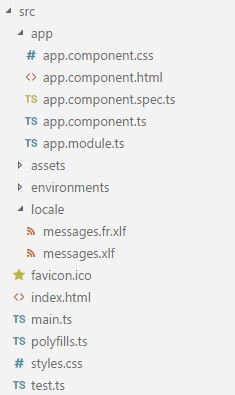
\includegraphics{intern.jpg}}
	\caption{project structure}
	\label{project structure}
\end{figure}
Note: update the package.json's script with below lines to run the application
\begin{lstlisting}[language=json, caption=package.json]
{
"start:fr": "ng serve --configuration=fr",
"build:fr": "ng build --configuration=fr",
"int:extract": "ng xi18n --output-path src/locale"
}
\end{lstlisting}
\chapter{Debugging}
\section{Debugging Extensions}
\subsection{Extensions}
\begin{itemize}
	\item{\href{https://augury.rangle.io/}{Augury Extension}}
	\item{\href{https://angular.io/guide/devtools}{Angular Devtools}}
\end{itemize}
\subsection{Debugging Angular Application in Visual Studio Code IDE}
\begin{enumerate}
	\item{In the VSC IDE, click on the left side of the editor and go to the Debug View menu. The launch.json file will store the debugging configuration. When debugging is being attempted fom here, for the first time, launch.json is not configured yet. VSC IDE will ask to create one. Click on Run and Debug option.}
	\item{Once Run and Debug is clicked, Select Environment dialog box will open. Type "Chrome" there and select.}
	\item{VSC IDE creates the \textit{launch.json} file with necessary configurations which can help in launching the application.}
	\item{Update port number to 4200 as the application would be running at 4200.}
	\item{If the \textit{launch.json} is already available in the VSC IDE, then choose the Add configuration option present within the Run and Debug dropdown.}
	\item{Run the application using \lstinline{ng serve --open} command}
	\item{Click of the left side of line number and add a breakpoint. Add as many breakpoints as needed. Once done, click on the green arrow to start debugging the application. The application launch happens in Google Chrome and the application’s execution will stop at the breakpoint number 1.}
\end{enumerate}
\textbf{Note:} Its key to execute and launch the application before the debugger is launched. This is because the debugger has to connect to a running instance of the application so that it can interact with it.

\chapter{Zone pollution}
\section{Intorduction}
Angular uses Zone.js as its signaling mechanism in order to detect when the application state changes. Zone.js can capture asynchronous operations like setTimeout, network requests, etc and Angular performs change detection based on signals from Zone.js.
Consider the below tasks or micro tasks:
\begin{itemize}
	\item{setTimeOut, setInterval}
	\item{Task or micro task scheduled by third party library}
\end{itemize}
These do not make any changes to data. Running change detection becomes unnecessary in such contexts. Hence in order to improve performance, its critical to recognise conditions when change detection is essentially not needed and then execute the code outside the Angular zone which can in turn avoid triggering redundant change detection calls.

Note: A zone in Angular is necessaily an execution context.

Zone pollution occurs when multiple zones are in use within the same Angular application. These can happen because of:
\begin{itemize}
	\item{Third party libraries: Some third party libraries may create their own zones which may conflict with Angular zone.}
	\item{Manual Zone creation: Developers may unknowingly create new zones if they are unware about zone handling by Angular.}
	\item{Integration with Non-Angular code: When integrating with non-Angular code, its important for developers to stay knowledgeful about how zones are managed to prevent pollution.}
\end{itemize}
\begin{lstlisting}[language=Typescript, caption=zone-pollution.component.ts]
import { Component, NgZone } from '@angular/core';
@Component({
	selector: 'app-zone-pollution',
	templateUrl: './zone-pollution.component.html',
	styleUrls: ['./zone-pollution.component.css']
})
export class ZonePollutionComponent {
	constructor(private ngZone: NgZone){}
	handleClick(){
		this.ngZone.run(()=>{
			// code here will run in Angular zone
			console.log('Button has been clicked');

		})
		setTimeout(()=>{
			// code here will in a different  zone
			console.log('setTimeout has been called');
		},1000)
	}
}
\end{lstlisting}
In the above example, 
\begin{itemize}
	\item{Inside handleClick(), ngZone.run() has been used to run code explicitly in Angular zone. This ensure Angular is aware of changes and change detection occurs.}
	\item{In the setTimeOut, however, code executes in a different separate zone and not Angular zone.}
\end{itemize}
This can lead to zone pollution. The outcome of the asynchronous tasks needs not be reflected in the Angular application state, they may not be detected or synchronized properly due to multiple zones. This is because of JavaScript’s event loop nature and this makes the code inside setTimeOut executes in a different zone.

Zone pollution can lead to unexpected behavior and make it quite difficult to track and debug issues. As an example, an asynchronous task initiated in different zone might not trigger Angular’s change detection which might result in UI inconsistencies. AngularDevTools can be used to detect unnecessary change detection.
Angular provides NgZone to explicitly run code in a specific zone. This comes in handy while integrating non-Angular code, particularly while using third-party libraries which are not designed keeping Zone.js in mind. Consider the below code:
\begin{lstlisting}[language=Typescript, caption=app.component.ts]
import { Component, NgZone, OnInit } from '@angular/core';
@Component(...)
class AppComponent implements OnInit {
  constructor(private ngZone: NgZone) {}
  ngOnInit() {
    this.ngZone.runOutsideAngular(() => setInterval(pollForUpdates), 500);
  }
}
\end{lstlisting}
Here, pollForUpdates is called in a zone outside Angular. Here, post the execution of the initialization logic, change detection will not get invoked inside the Angular zone, but will be invoked outside the Angular zone and hence change detection will get skipped.
\chapter{Slow Computations}
When change detection cycle runs, Angular will synchronously, 
\begin{itemize}
	\item{Assess all the template expressions for all the components, unless stated explicitly. This is performed on the basis of the change detection strategy that has been configured for that component}
\item{Assess the life cycle hooks like ngDoCheck, ngAfterViewChecked, ngAfterContentChecked and ngOnChanges. Since Angular runs computations in a sequential manner, with just a single slow computation within a template or a lifecycle hook, it can completely slow down the complete change detection process.}
\end{itemize}
Angular DevTool’s profiler can be used to indetify heavy computations, so that needful actions can be taken.
Slow computations can be avoided by following the below strategies:

\begin{itemize}
	\item{Optimization of the underlying algorithm: Effort can be put in to speed up the algorithm that seems to be causing slowness. This is suggested approach.}
	\item{Using pure pipes to cache: Heavy computations can be moved a pure pipe. This can surely prove to be helpfu as Angular performs reevaluation of a pure pipe only when changes to input to the pipe gets detected, that too, by comparing it to the previous invocation by Angular. }
	\item{Usage of memoization: Memoization technique is a similar to pure pipes. The difference is that pure pipes keeps only the latest result from the computation whereas memoization can store multiple results.}
	\item{Avoiding repaints/reflows in lifecycle hooks: Reflows and repaints are generally very slow. So its advisable to avoid doing these in every single change detection cycle.}
\end{itemize}

\chapter{Skipping Component subtrees}
\section{Understanding skipping component subtrees}
\subsubsection*{Why there is need to skip component subtrees?}
Change detection happens necessarily very fast for most of the applications. However, there can be scenarios when an application has a remarkably large component tree. It can so happen that a certain part of the application is actually not much affected by a state change. However, as per norms, Angular will make change detection to run across the entire application. This can result in performance issues.
\subsubsection*{What does skipping component subtrees mean?}
If a certain part of the application doesn’t seem to be affected by a state change, then the change detection associated with the entire component subtree can be skipped by making use of OnPush.

With OnPush change detection, Angular is instructed to perform change detection for a component subtree only when:
\begin{itemize}
	\item{A new input is received by the root component as a result of a template binding. The current and past value of the input is compored using == by Angular.}
\item{An event is handled by Angular (for example usage of event binding, output binding, or @HostListener ) in the subtree's root component or any of its children if they have used OnPush change detection or not.}
\end{itemize}

\subsubsection*{Using OnPush}
Change detection strategy of a component can be set to OnPush within the @Component decorator.

\begin{lstlisting}[language=Typescript]
import { ChangeDetectionStrategy, Component } from '@angular/core';
@Component({
  changeDetection: ChangeDetectionStrategy.OnPush,
})
export class MyCustomComponent {}
\end{lstlisting}

Let us look at how Change Detection happens in specific scenarios.

\begin{itemize}
	\item Scenario1:
For a component tree where OnPush is not mentioned, Angular performs change detection for the entire component tree as usual. For components having OnPush configured, change detection is skipped until the component gets new inputs.

\begin{figure}[h]
	\centerline{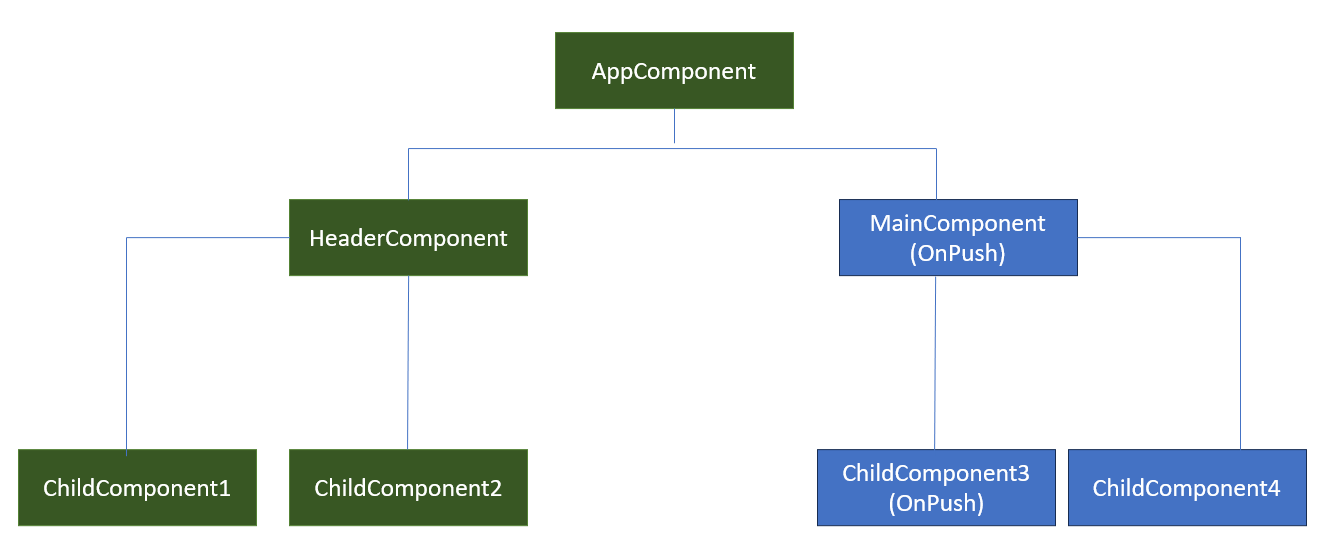
\includegraphics[scale=.5]{onpush11695758391262.png}}
	\caption{Scenario 1}
	\label{Scenario 1}
\end{figure}
Green ones will be checked by Angular.

\item Scenario2:
When Angular has to handle an event within a component for which OnPush strategy is configured, Angular will execute change detection inside the entire component tree. Component subtrees having OnPush will be ignored, until new inputs are received. 

\begin{figure}[h]
	\centerline{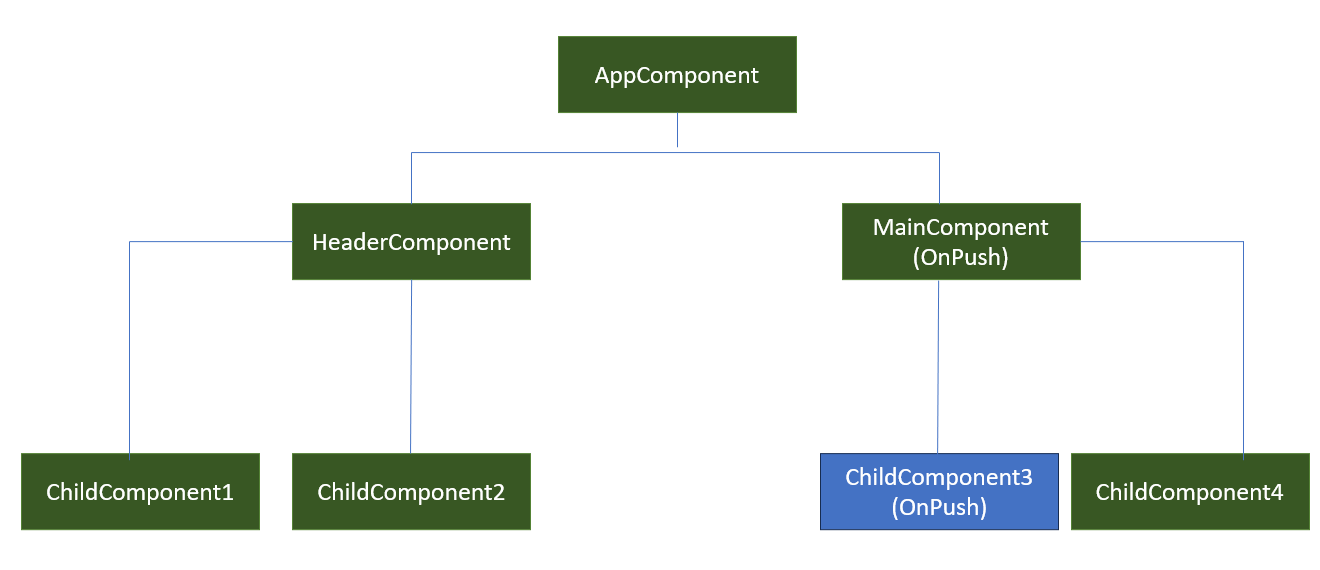
\includegraphics[scale=.5]{onpush21695758405033.png}}
	\caption{Scenario 2}
	\label{Scenario 2}
\end{figure}
\item Scenario3:

When Angular has to handle an event withing a component for which OnPush has been configured, Angular will execute change detection inside the entire component tree, including the ancestors of the component.

\begin{figure}[h]
	\centerline{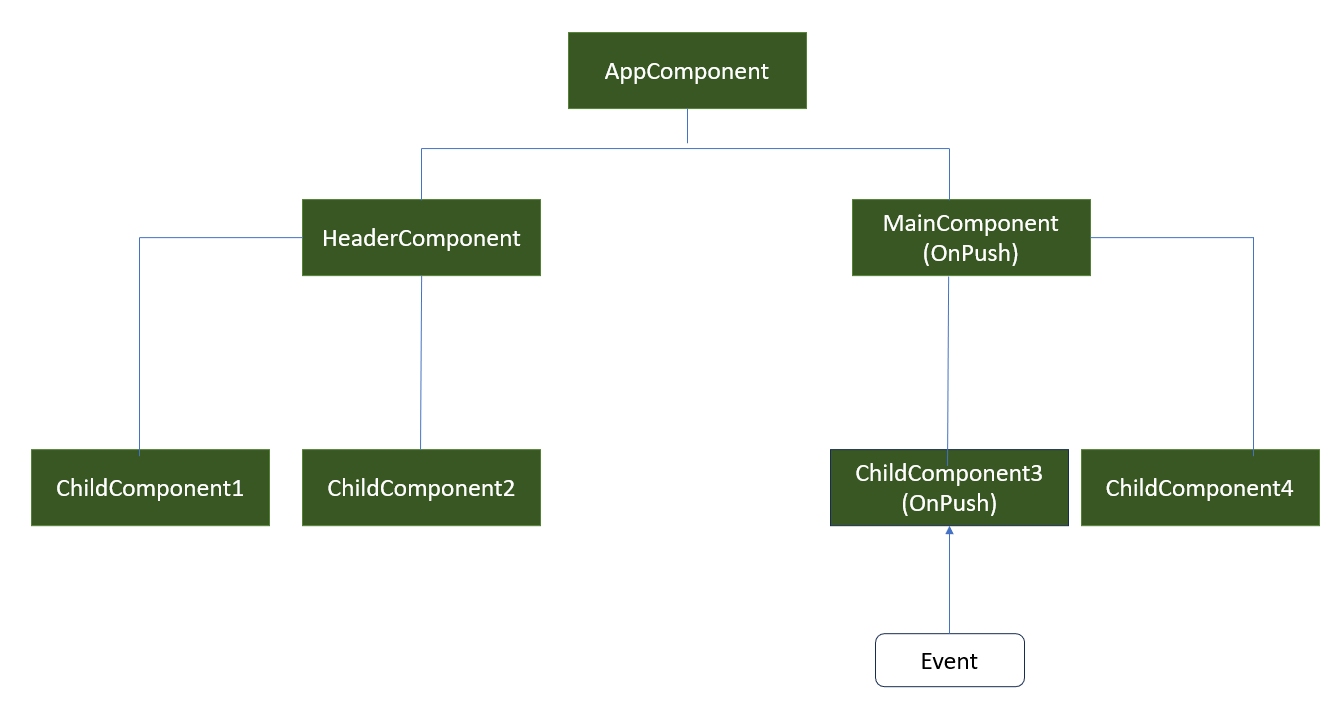
\includegraphics[scale=.5]{onpush31695758418442.png}}
	\caption{Scenario 3}
	\label{Scenario 3}
\end{figure}

\item Scenario4:
When parent passes new input to child component having OnPush, Angular will run change detection in child component as it received new inputs. But for further grand children where OnPush is configured, Angular will not run change detection unless it receives new inputs as well.

\begin{figure}[h]
	\centerline{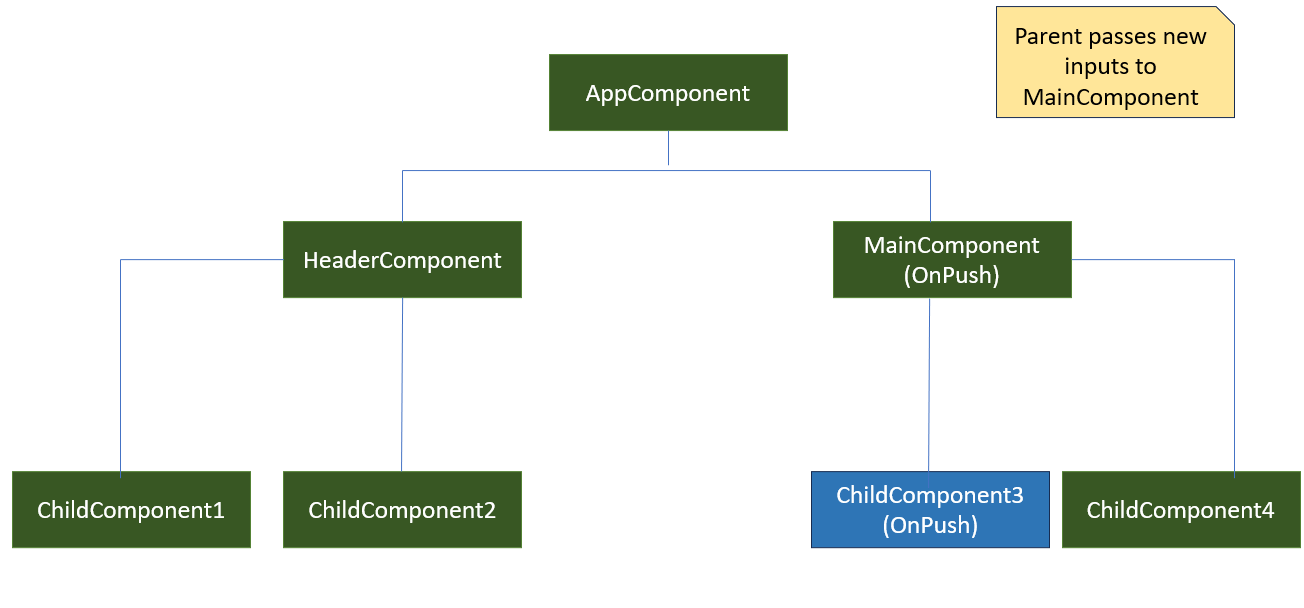
\includegraphics[scale=.5]{onpush41695758431278.png}}
	\caption{Scenario 4}
	\label{Scenario 4}
\end{figure}
\end{itemize}

\appendix

\end{document}

%\begin{lstlisting}[caption=example.ts, language=Typescript]
%\end{lstlisting}


%\begin{figure}[htbp]
%	\centerline{\includegraphics[scale=.5]{}}
%	\caption{}
%	\label{}
%\end{figure}

%h: here, where the figure appears in the text (use can always just use [h] )
%t: top,  top of the current page.
%b: bottom of the current page.
%p: page, top of the next available float space (sometimes end up being the end of the document).


% https://researchguides.njit.edu/latex/figures
% https://users.ece.utexas.edu/~garg/dist/listings.pdf
% https://uva-fnwi.github.io/LaTeX/extra1/Tikz/
% https://lex.infosysapps.com/web/en/app/toc/lex_auth_0127668079785820163566/overview
